% ══════════════════════════════════════════════════════════════════════════════
\section{Numerical Experiments}
\label{sec:experiments}
% ══════════════════════════════════════════════════════════════════════════════

All experiments use $h = J = -1.0$, $\delta t = 0.1$,
$\epsilon_{\mathrm{cut}} = 10^{-11}$, and float32 precision,
unless otherwise noted.
Although $\epsilon_{\mathrm{cut}} = 10^{-11}$ lies below the float32 noise
floor ($\varepsilon_{\mathrm{mach}} \approx 10^{-7}$), it is compatible with
float32 arithmetic because LAPACK \texttt{SGESVD} returns singular values
as float32 scalars representable down to $\sim10^{-38}$, and the threshold is
applied as a relative comparison $s_i \geq \epsilon_{\mathrm{cut}}\,s_0$.
In practice, all physically meaningful singular values lie well above
$10^{-7}\,s_0$; the cutoff acts only to discard subnormal numerical zeros
produced by rounding, leaving $\chimax$ as the active truncation constraint
in every experiment.
The center observable is $Z_c$ at site $(\lfloor(N_x-1)/2\rfloor,\lfloor(N_y-1)/2\rfloor)$,
the geometric center of the grid.

The primary observable throughout is the \emph{spin autocorrelation function}
\begin{equation}
 C(t) = \frac{1}{2^N}\,\mathrm{Tr}\bigl[Z_c(t)\,Z_c\bigr],
 \qquad
 Z_c(t) = e^{i\mathcal{H}t}\,Z_c\,e^{-i\mathcal{H}t},
 \label{eq:ct_def}
\end{equation}
where $N$ is the number of sites and $Z_c$ is the Pauli-$Z$ operator at the
lattice center.
$C(t)$ measures the overlap between the Heisenberg-evolved operator $Z_c(t)$
and its initial form $Z_c$: it equals 1 at $t=0$ by normalization, and
decreases toward 0 as $Z_c(t)$ scrambles into many-body Pauli strings
that are orthogonal to $Z_c$.
This decay is purely \emph{unitary} --- there is no dissipation or energy loss;
$C(t) \to 0$ means the operator has spread across the entire lattice,
not that it has decayed.

\subsection{Correctness Validation}
\label{sec:correctness}

Validation proceeds on two levels.
The first establishes \emph{implementation correctness} by comparison with an
existing reference implementation.
The second establishes \emph{physical fidelity} through consistency with
predictions derived independently of any code.
This second level is not a cross-check of an existing answer: it is the
instrument through which the physical behavior of the system was understood,
and through which the results of \S\ref{sec:bp_convergence} --- including the
connection between operator-placement symmetry and BP fixed-point multiplicity
--- were discovered.
The distinction matters: where the reference begins from adapted library codes,
the implementation reported here codes the physics directly --- each component
derived from first principles and validated against the physical predictions it
is designed to satisfy.

\medskip
\noindent\textbf{Implementation correctness} is established against two external references:
\begin{enumerate}
 \item \textbf{Julia reference}: $\Ct$ for $4\times4$ at $\chi=50$ matches the
 Julia float64 implementation to within float32 rounding
 ($<10^{-6}$ absolute error) for $t \leq 1.6$.
 \item \textbf{Chi consistency}: for $t \leq 1.4$, $\Ct$ agrees across
 $\chi \in \{40, 50, 60, 80, 110\}$ to 5 significant figures
 (Figures~\ref{fig:ct_4x4} and~\ref{fig:ct_5x5}), confirming that truncation error is negligible
 for early-to-mid time evolution at these bond dimensions.
\end{enumerate}

\medskip
\noindent\textbf{Physical fidelity} is established by consistency with predictions
derived independently of any code.
The simulation is correct not only when it matches a reference, but when it
reproduces the qualitative and quantitative behavior that the physics demands.
\begin{enumerate}
 \item \textbf{Operator spreading and lightcone}: under unitary evolution,
 $Z_c(t)$ must spread outward from the center site.
 The non-identity Pauli weight $n(r,t)$ should grow from a single pixel
 at $t=0$ to a spatially extended pattern, bounded by the Lieb--Robinson
 cone~\citep{liebrobinson}.
 The simulation reproduces this: $n(r,t)=0$ at all non-center sites at
 $t=0$, and the spreading front reaches the lattice boundary at
 $n^*$ layers (Table~\ref{tab:lightcone}), consistent with the predicted
 lightcone velocity.
 \item \textbf{Early-time universality}: for $t \leq 1.4$ the operator front
 has not yet reached any lattice boundary regardless of grid size, so
 $\Ct$ must be independent of both $\chi$ and grid size.
 All eight $\chi$ values and all eight grid sizes agree to 5 significant
 figures in this regime (Figures~\ref{fig:ct_4x4} and~\ref{fig:ct_5x5}; Table~\ref{tab:ct_grids}).
 \item \textbf{$C_4$ symmetry of $n(r,t)$}: placing $Z_c$ at the geometric
 center of an odd grid imposes $C_4$ symmetry on the operator lightcone.
 The simulation reproduces exact four-fold symmetry in $n(r,t)$ at every
 Trotter layer, to 6 significant figures in all corner weights --- a
 sensitive check that the center formula, gate application, and BP update
 are all implemented correctly.
 \item \textbf{Scrambling to zero}: at long times, $Z_c(t)$ spreads into
 many-body Pauli strings orthogonal to $Z_c$, so $\Ct \to 0$.
 The simulation reaches $\Ct < 10^{-3}$ by $t \approx 4$ on all grids
 large enough to avoid finite-size reflections, and $n(r,t)$ saturates
 uniformly across all sites, both consistent with full operator scrambling.
\end{enumerate}
These physical consistency checks validate aspects of the simulation that
numerical comparisons alone cannot reach: a wrong center formula or a broken
symmetry in the gate implementation would violate items~3 and~1 respectively,
even if $\Ct$ happened to match a reference at early times.

\paragraph{Runtime diagnostic measures.}
Agreement with the Julia reference and chi consistency together confirm that
$\Ct$ is correct when the simulation runs cleanly.
However, $\Ct$ alone cannot distinguish a correct answer from a physically
plausible artifact: a BP trap or an over-saturated bond dimension can produce
a smooth, monotone $\Ct$ trajectory that deviates from the true value by
$5$--$10\%$ without any obvious signature in $\Ct$ itself.
To detect such failures before they corrupt the result, \textsc{CppSim} reports
four auxiliary diagnostics per Trotter layer, listed in
Table~\ref{tab:diagnostics}.

\begin{table}[ht]
\small\centering
\caption{Runtime diagnostic measures reported per Trotter layer,
 spanning the full failure chain: truncation $\to$ BP $\to$
 Bethe approximation $\to$ bond capacity.}
\label{tab:diagnostics}
\begin{tabular}{lll}
\toprule
Quantity & Definition & Failure signal \\
\midrule
\texttt{gate\_err} &
 $\sum_{\text{bonds}} \sum_{i>\chi} s_i^2 \,/\, \sum_i s_i^2$ &
 $> 10^{-1}$: $\Ct$ qualitative only \\
Bethe norm &
 $\exp\!\bigl(\sum_v \log f_v - \sum_e \log Z_e\bigr)$ &
 $\geq 2.0$: \texttt{norm\_exploded} flag \\
BP sweeps\,/\,$\delta$ &
 iterations to $\max_e|\Delta\mu_e| < \epsilon_{\mathrm{tol}}$ &
 sweeps\,$\geq 30$ \& $\delta < \epsilon_{\mathrm{tol}}$: trapped layer (\S\ref{sec:bp_convergence}) \\
$S_e / \log\chi$ &
 $-\sum_k \lambda_k^2 \log\lambda_k^2 \,/\, \log\chi$ &
 $\geq 0.5$: increase $\chi$, not $\alpha$ (BP damping, \S\ref{sec:bp_convergence}) \\
\bottomrule
\end{tabular}
\end{table}

The four diagnostics address distinct points in the simulation pipeline.
\texttt{gate\_err} captures SVD truncation at the gate level: it is the
fraction of singular value weight discarded by the $\chi$ cutoff, summed
over all bonds in the layer.
A value below $10^{-2}$ means truncation is not the limiting factor;
values above $10^{-1}$ (seen at $\chi=20$ on large grids) signal that
$\Ct$ is qualitative rather than quantitative.
The Bethe norm measures the self-consistency of the BP environment:
it equals 1 exactly on a tree and deviates when the Bethe approximation
breaks down on the loopy graph --- a graph containing cycles, where BP is an
approximation rather than exact~\citep{yedidia2005constructing}.
Values above 2.0 trigger the \texttt{norm\_exploded} flag and typically
correlate with incorrect $\Ct$; the norm can recover spontaneously in the
next layer as BP re-converges, so a transient spike does not necessarily
invalidate the run.
The BP sweep count and final $\delta$ jointly identify convergence quality:
the combination (sweeps $\geq 30$, $\delta < \epsilon_{\mathrm{tol}}$) is the
early-warning signature of BP converging to a wrong fixed point --- a
\emph{trapped layer}, analyzed in detail in \S\ref{sec:bp_convergence}.
Finally, $S_e / \log\chi$ is the per-bond entanglement saturation fraction,
where $S_e = -\sum_k \lambda_k^2 \log\lambda_k^2$ is the operator-space
entanglement entropy (OSEE) of the Vidal singular values on bond $e$.
When $S_e / \log\chi \geq 0.5$, the bond is more than half-saturated and
the variational manifold at bond dimension $\chi$ is approaching its capacity;
increasing the BP damping factor $\alpha$ cannot compensate, and increasing $\chi$ is the only remedy
(\S\ref{sec:bp_convergence}, capacity boundary).

% ── Chi convergence figures and trap table ────────────────────────────────────
\subsection{$\chi$-Convergence of $C(t)$}
\label{sec:chi_convergence}

Throughout this section, GPU-B denotes the 32\,GB, 1.2\,TB/s configuration
and GPU-A the 32\,GB, 1.0\,TB/s configuration
(Section~\ref{sec:portability}).
Figures~\ref{fig:ct_4x4} and~\ref{fig:ct_5x5} show $\Ct$ for $\chi \in
\{20,\ldots,100\}$ on $4\times4$ and $5\times5$ grids (GPU-B), comparing
Householder QR (solid lines) against Adaptive QR (dashed lines).

\begin{figure}[ht]
\centering
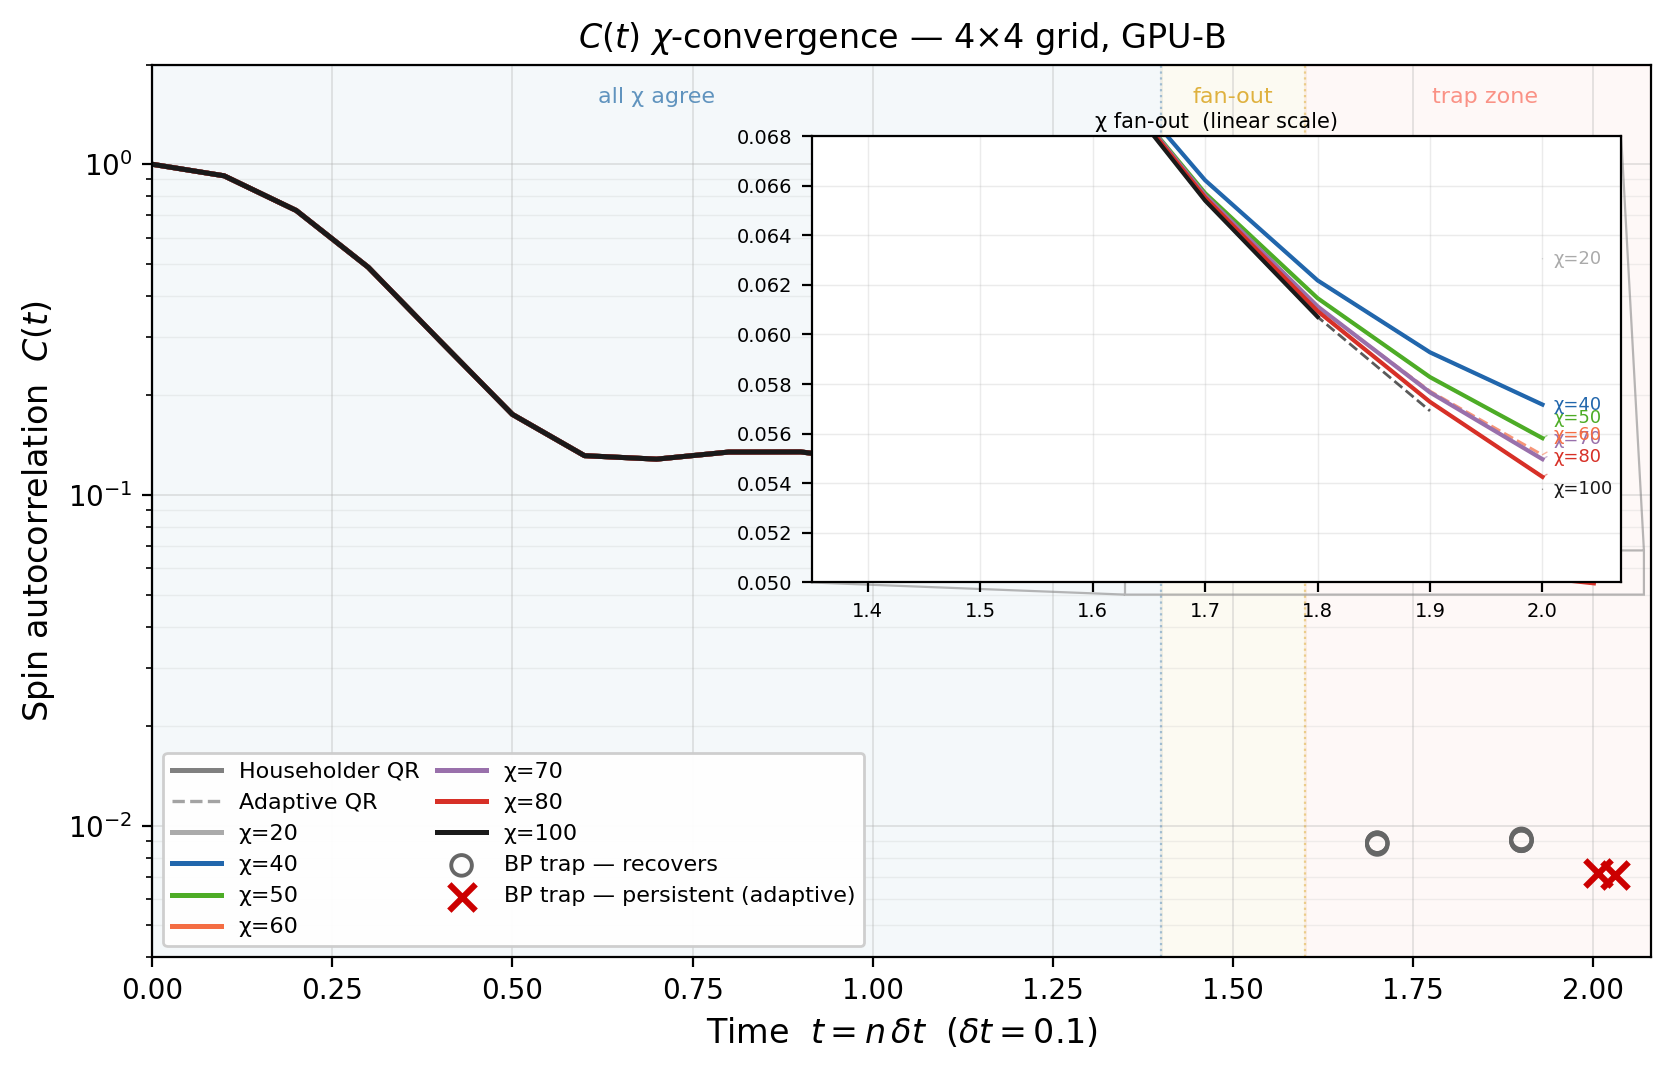
\includegraphics[width=\linewidth]{fig_ct_4x4.png}
\caption{%
 Spin autocorrelation $\Ct$ on a $4\times4$ grid (GPU-B, log scale) for
 $\chi \in \{20, 40, 50, 60, 70, 80, 100\}$.
 Householder QR: solid lines. Adaptive QR: dashed lines (same color per $\chi$).
 Three dynamical regimes are shaded:
 \emph{all $\chi$ agree} ($t \leq 1.4$, both methods overlap to 5 significant
 figures);
 \emph{fan-out} ($1.4 < t \leq 1.6$, $\chi$-dependent truncation error becomes
 visible, detail in inset);
 \emph{trap zone} ($t > 1.6$, BP metastable traps may occur).
 Open circles: BP traps that recover at the next layer (Householder QR).
 Red crosses: persistent traps that do not recover by $t=2.0$ (Adaptive QR,
 $\chi=70$ and $\chi=100$).
 Inset (linear scale): late-time $\chi$ fan-out with per-$\chi$ labels;
 Householder convergence is monotone from $\chi=40$ to $\chi=100$,
 extrapolating to $\Ct(2.0) \approx 0.052$--$0.053$.}
\label{fig:ct_4x4}
\end{figure}

\begin{figure}[ht]
\centering
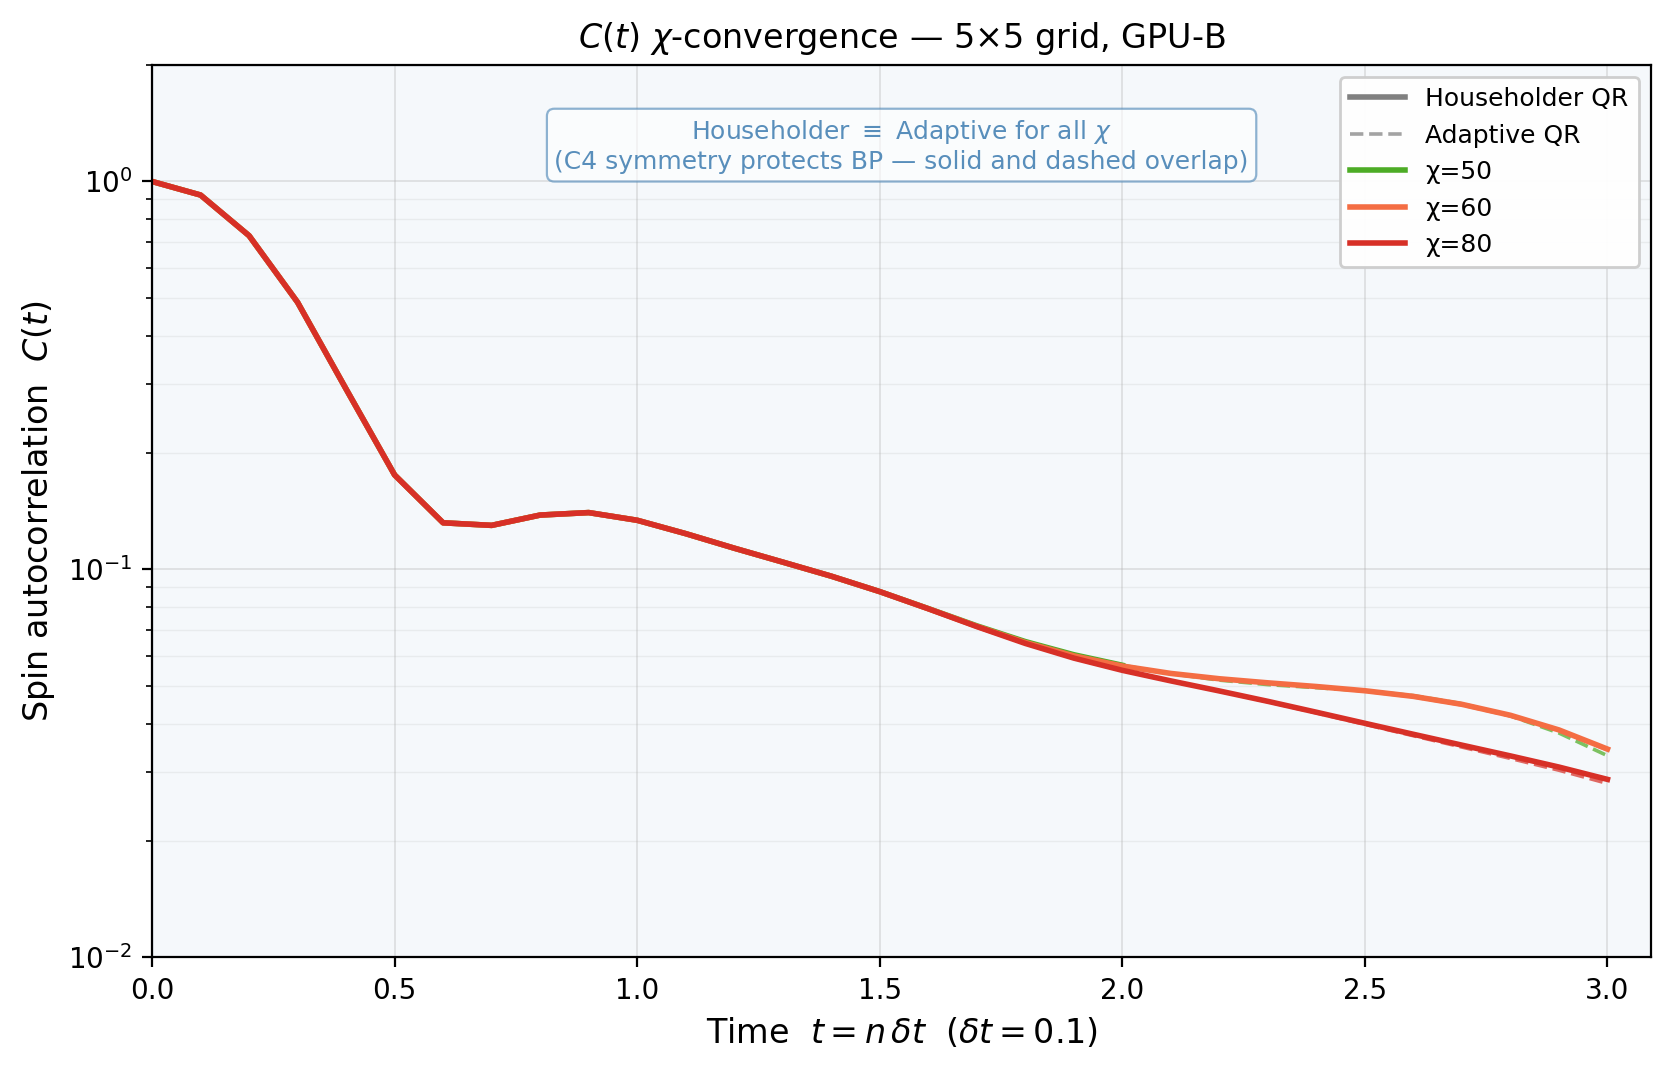
\includegraphics[width=\linewidth]{fig_ct_5x5.png}
\caption{%
 Spin autocorrelation $\Ct$ on a $5\times5$ grid (GPU-B, log scale) for
 $\chi \in \{50, 60, 80\}$, 30 Trotter layers.
 Householder QR: solid lines. Adaptive QR: dashed lines.
 The two methods are indistinguishable at every layer: the C4 lattice symmetry
 of the centered initial condition prevents BP from finding metastable fixed
 points regardless of gauge, so Adaptive QR produces identical physics to
 Householder QR on this geometry.
 The $\chi$-convergence is slower than on $4\times4$: curves for $\chi=50$,
 $60$, and $80$ remain visibly separated at $t=3.0$, consistent with larger
 entanglement growth on the bigger grid.}
\label{fig:ct_5x5}
\end{figure}

The $4\times4$ results reveal three regimes:

\paragraph{Early time ($t \leq 1.4$): universal agreement.}
All $\chi$ values and both QR modes agree to 5 significant figures,
confirming that bond dimension plays no role until entanglement saturates the
smallest bond.

\paragraph{Monotone convergence for clean runs ($t > 1.4$).}
The Householder convergence curve is strictly decreasing in $\chi$ at every
late layer.
At $t=2.0$: $\Ct(\chi=40) > \cdots > \Ct(\chi=100)$, with values
$0.0572 > 0.0558 > 0.0552 > 0.0550 > 0.0543$,
extrapolating to $\approx 0.052$--$0.053$.
We identify $\chi^* \approx 60$ as the point of diminishing returns:
below it each increment in $\chi$ buys meaningful accuracy; above it the gain
is less than $0.2\%$ per step while cost grows as $\chi^4$.

\paragraph{Trap zone ($t > 1.6$).}
BP metastable traps appear stochastically.
Householder traps are transient --- they recover at the next layer and do not
contaminate the $\chi$-convergence curve.
Adaptive traps at $\chi=70$ and $\chi=100$ are persistent at $t=2.0$
(final layer), producing $\Ct \approx 0.007$ instead of $\approx 0.055$.

Table~\ref{tab:trap_inventory} catalogues all observed BP traps across both
grids, QR modes, and GPU architectures.

\begin{table}[ht]
\centering
\caption{BP trap inventory: layer indices where $\Ct$ collapsed to
 $\approx 0.007$--$0.010$, and whether the trap recovered at the next layer.
 \emph{Recovers}: correct value restored at layer $+1$.
 \emph{Persistent}: final layer still trapped, no further chance to recover.
 GPU-A runs (both QR modes) show more trapping than GPU-B at the same $\chi$ due to
 floating-point non-determinism (matrix multiply-accumulate units (GPU-B) versus scalar vector-ALU (GPU-A)).
 \emph{n/a}: that $\chi$ was not run on this architecture/mode combination.
 No traps occur on the $5\times5$ grid in either method.}
\label{tab:trap_inventory}
\small
\begin{tabular}{cllll}
\toprule
$\chi$ & GPU-B Adaptive & GPU-B Householder & GPU-A Adaptive & GPU-A Householder \\
\midrule
20 & --- & L17, L19 (recover) & L17 (recovers) & L17, L19 (recover) \\
40 & --- & --- & n/a & --- \\
50 & --- & --- & L20 (\textbf{persistent}) & L19 (\textbf{persistent}) \\
60 & --- & L19 (recovers) & n/a & L12--L20 (\textbf{persistent}) \\
70 & L20 (\textbf{persistent}) & L17 spike (recovers) & n/a & L6, L16, L19, L20 (\textbf{persistent}) \\
80 & --- & --- & L16, L18, L20 (\textbf{persistent}) & --- \\
90 & n/a & L19 (recovers) & n/a & n/a \\
100 & L20 (\textbf{persistent}) & L19 (recovers) & n/a & n/a \\
\midrule
\multicolumn{5}{l}{\emph{$5\times5$, all $\chi$}: no traps in either method (C4 symmetry protects BP).} \\
\bottomrule
\end{tabular}
\end{table}

% ── BP fixed-point section ────────────────────────────────────────────────────
\subsection{BP Fixed-Point Multiplicity, Root Cause, and Trap Remediation}
\label{sec:bp_convergence}

Figure~\ref{fig:ct_4x4} shows isolated anomalous layers --- marked with open circles
and red crosses --- where $\Ct$ collapses to $\approx 0.007$--$0.009$ while all
neighboring layers follow the smooth converging sequence.
These \emph{trapped layers} are symptoms of a deeper structural property of the
BP fixed-point landscape.
Before presenting the experimental data, we define the two distinct ways BP can
fail, since both appear in the results and must not be confused.

\paragraph{Two failure modes.}
\emph{Type~1 --- metastable trap (trapped layer)}: BP converges in a finite
number of sweeps ($\delta < \epsilon_{\mathrm{tol}} = 10^{-5}$), yet $\Ct$
collapses to $\approx 0.007$--$0.010$, inconsistent with all neighboring layers.
In optimization terms, the iterative message-passing dynamics have settled into
a local basin of the Bethe free energy landscape --- a local fixed point that is
stable under further BP iteration but is not the global optimum.
The word \emph{trap} captures this precisely: the algorithm is not diverging;
no amount of additional sweeps at the same $\alpha$ will escape the basin.
The sweep count at a trapped layer is $2$--$3\times$ the typical value
(e.g., 49 sweeps at $\chi=110$, $t=1.7$ versus 12--18 on neighboring layers),
providing an early-warning signal detectable at runtime.

\emph{Type~2 --- non-convergence}: BP exhausts the 100-sweep budget with
$\delta \gg \epsilon_{\mathrm{tol}}$.
The resulting $\Ct$ is unreliable at that layer, but the next Trotter layer
typically recovers; the event is self-announcing (sweep count $= 100$, large
$\delta$).
Type~2 does not imply a wrong answer: GPU-A $\chi=50$, $t=1.9$ fails to
converge (100 sweeps, $\delta = 1.80\times10^{-5}$) yet produces $\Ct = 0.060$,
agreeing with the GPU-B clean run to within 3\%.

The sweep count alone does not distinguish the types; the final $\delta$ is
essential.
A runtime diagnostic should flag any layer where (sweeps $\geq 30$) \emph{and}
($\delta < \epsilon_{\mathrm{tol}}$) as a candidate Type~1 trapped layer,
warranting a retry.
With this vocabulary in place, we now identify the root cause.

\paragraph{Root cause: operator-placement symmetry governs fixed-point multiplicity.}
When $Z_c$ is placed at the geometric center of an odd grid, the operator
lightcone has exact $C_4$ symmetry from the first Trotter layer: all four
quadrants of the lattice are equivalent, so symmetry-equivalent bonds carry
identical Schmidt spectra and BP messages at the correct fixed point must also
be equal.
This constraint \emph{collapses} the effective degrees of freedom that BP must
resolve, reducing the number of competing fixed points in the Bethe free energy
landscape.
Breaking this symmetry --- by displacing $Z_c$ even one site, or by using a
grid geometry where no site achieves true $C_4$ symmetry --- lifts the
constraint, populating the message manifold with additional local minima and
making traps more likely.

We test this hypothesis with a $5\times5$ grid, where the geometric center
$(2,2)$ achieves exact $C_4$ symmetry (all four corners at Manhattan distance
$d_{\max}=4$), unlike the $4\times4$ grid where no center site achieves this.
The experiment runs $\chi \in \{20, 40, 60, 80, 100\}$ on the $5\times5$
symmetric grid and compares to the $4\times4$ results (Table~\ref{tab:trap_inventory}).

The result is \emph{zero} Type~1 trapped layers on the symmetric $5\times5$ grid
across all $\chi$ values and all layers (Figure~\ref{fig:ct_5x5}),
with final values $\Ct(\chi=20)=0.000716$, $\Ct(\chi=40)=0.000907$,
$\Ct(\chi=60)=0.001073$, $\Ct(\chi=80)=0.028089$, $\Ct(\chi=100)=0.042065$.
The $5\times5$ grid has strictly more loops ($40$ bonds versus $24$ for $4\times4$),
and the data in Table~\ref{tab:trap_inventory} already show
that larger grids and higher bond dimensions increase the complexity of the BP
update and the density of the entanglement spectrum.
One might therefore expect more trapped layers on the $5\times5$ grid, not
fewer.
Symmetry proves to be the dominant factor: on the symmetric grid, BP sweeps
produce only Type~2 non-convergence events at high saturation
($S_e/\log\chi \gtrsim 0.65$, late layers, $\Ct \approx 0$) --- self-announcing
events that do not corrupt $\Ct$ --- but never settle into a wrong fixed point.
At $\chi=80$, the trap that struck at $t=1.7$ on the $4\times4$ grid
($\Ct=0.0088$) is entirely absent: the $5\times5$ symmetric run at $t=1.7$
gives $\Ct=0.071$ with $11$ sweeps, physically consistent with all neighbors.

The mechanism is as follows.
On a $C_4$-symmetric lattice with a $C_4$-symmetric initial operator, the
correct BP fixed point respects the symmetry: messages on related bonds are
equal.
This symmetry-constrained fixed point is unique in the symmetric subspace.
When the operator breaks $C_4$ symmetry, the full (unsymmetrized) message
manifold is active, and multiple local minima can coexist at the same $(\chi,
t)$.
The floating-point arithmetic path --- determined by GPU reduction order ---
then selects among them, producing the architecture-dependent, non-monotone
trap patterns observed on the $4\times4$ grid.

\paragraph{Further evidence: architecture and update-rule experiments.}
Two additional controlled experiments corroborate the fixed-point multiplicity
picture on the $4\times4$ grid.

\emph{Cross-architecture experiment.}
The trap patterns in Table~\ref{tab:trap_inventory} are \emph{complementary} across
architectures: GPU-B traps at $(\chi=80,\,t=1.7)$ and $(\chi=70,\,t=2.0)$
while GPU-A is clean at those points; conversely, GPU-A traps at
$(\chi=50,\,t=2.0)$ and $(\chi=80,\,t=2.0)$ while GPU-B is clean.
Both GPUs execute the same algorithm in float32, but matrix multiply-accumulate units (GPU-B) and
scalar vector-ALU (GPU-A) reduction trees differ in rounding order,
perturbing the message trajectory enough to select a different basin.
When both are un-trapped, $\Ct$ agrees to within $1$--$2\times10^{-3}$.

\emph{Update-rule experiment.}
Fixing $\chi=80$ on GPU-B, we compare undamped BP ($\alpha=1$) and damped BP
with $\alpha \in \{0.50,\, 0.80\}$.
Damping introduces a momentum term into the message update:
\begin{equation}
 \mu_e^{(k+1)}
 \;\leftarrow\;
 (1-\alpha)\,\mu_e^{(k)} \;+\; \alpha\,\hat{\mu}_e^{(k+1)},
 \label{eq:damping}
\end{equation}
where $\hat{\mu}_e^{(k+1)}$ is the undamped update.
Spectrally, damping maps an eigenvalue $\lambda$ of the BP Jacobian to
$(1-\alpha) + \alpha\lambda$, compressing the spectrum toward 1 and
suppressing oscillatory modes that otherwise overshoot the fixed point.
The result at $(\chi=80, t=1.7)$: $\alpha=0.50$ avoids the trap entirely
($\Ct = 0.066$), while $\alpha=0.80$ and undamped both find the wrong basin
($\Ct = 0.009$, identical to six decimal places).
At $(\chi=80, t=1.9)$: the roles reverse --- $\alpha=0.80$ finds the correct
fixed point ($\Ct = 0.057$) while $\alpha=0.50$ does not converge.
Both experiments are consistent with the symmetry picture: the $4\times4$ grid
has multiple fixed points, and any perturbation to the message trajectory
(architecture, damping) selects among them.

\paragraph{Trap remediation.}
A key practical conclusion is that traps are \emph{not fatal}: the correct
$\Ct$ can be recovered by retrying the BP step with a different $\alpha$.
This is confirmed by the cross-$\alpha$ experiment: GPU-B damped $\alpha=0.50$
at $(\chi=80, t=1.7)$ recovers $\Ct = 0.066$, matching GPU-A undamped
($\Ct = 0.066$) to within $1.5\times10^{-3}$ --- two different hardware paths
arriving at the same physical fixed point.
The most robust long-term remedy is to use a symmetric initial condition
(odd grid with $Z_c$ at the geometric center), which eliminates Type~1 traps
entirely.
For asymmetric configurations, the remediation procedure is:
\begin{enumerate}
 \item After each BP run, check whether (sweeps $\geq 30$) and
 (delta $< \epsilon_{\mathrm{tol}}$).
 If so, flag as candidate Type~1 trap.
 \item Verify by comparing $\Ct$ to the previous layer: a drop of $>50\%$
 with no corresponding increase in \texttt{gate\_err} is a strong signal.
 \item Retry BP with a different $\alpha$ (e.g., try $\alpha=0.50$ if
 undamped trapped; try $\alpha=0.80$ if $\alpha=0.50$ trapped).
 \item If all $\alpha$ values fail simultaneously, the bond dimension is
 insufficient: increase $\chi$ rather than tuning $\alpha$.
\end{enumerate}

\paragraph{Capacity boundary.}
A distinct third regime appears at high entanglement saturation
($S_e/\log\chi \gtrsim 0.65$, observed consistently across both grid sizes):
BP non-convergence (Type~2) becomes systematic and $\Ct$ approaches zero
regardless of $\alpha$.
At these layers the bond dimension itself is the bottleneck --- the variational
manifold is saturated and no message-passing strategy can compensate.
This boundary is cleanly separated from the fixed-point multiplicity regime:
in the multiplicity regime, at least one $\alpha$ recovers the correct $\Ct$;
at the capacity boundary, none does.
The appropriate response is to increase $\chi$, not to tune the update rule.

At $\chi=40$ and $\chi=60$, both GPU-B and GPU-A are trap-free and agree to
within $5\times10^{-4}$ ($\Ct(\chi=60, t=2.0)$: GPU-B $= 0.0551$,
GPU-A $= 0.0546$), confirming these as \emph{portable operating points}: the BP
landscape is simple enough that neither damping nor architecture choice matters.
The $5\times5$ symmetric runs confirm that portability extends beyond
$\chi=60$: on a symmetric grid, $\chi=80$ and $\chi=100$ are also trap-free,
suggesting that the portable range expands when physical symmetry is respected.

% ── Operator spreading and lightcone ─────────────────────────────────────────
\subsection{Operator Spreading and Lightcone Saturation}
\label{sec:lightcone}

The spin autocorrelation $\Ct = \mathrm{Tr}[Z_c(t)\,Z_c]/2^N$ measures how
much the evolved operator $Z_c(t)$ still overlaps its initial form $Z_c$ at
the center site.
Under unitary evolution, $\Ct \to 0$ does \emph{not} signal dissipation:
there is no energy loss, no bath.
Instead it signals \emph{operator scrambling}: $Z_c(t)$ has spread across
the lattice into many-body Pauli strings that are orthogonal to the initial
local $Z_c$.
The rate and geometry of this spreading are constrained by a Lieb--Robinson
bound~\citep{liebrobinson}: the operator front propagates at a group velocity
bounded by $v_{\mathrm{LR}} = 2|J|$ for the Heisenberg coupling
(equation~\eqref{eq:hamiltonian}), reaching the lattice corner at Manhattan
distance $d_{\mathrm{max}}$ after at least
\begin{equation}
 n^* = \frac{d_{\mathrm{max}}}{2|J|\,\delta t}
 \quad \text{Trotter layers,}
 \label{eq:nstar}
\end{equation}
where $\delta t$ is the Trotter step size.
In all experiments here $|J| = 1$ and $\delta t = 0.1$, so
$n^* = 5\,d_{\mathrm{max}}$.
For $n < n^*$, the boundary has not yet been reached and $\Ct$ probes
bulk scrambling; for $n \geq n^*$, finite-size effects enter and $\Ct$
approaches its long-time plateau.
Table~\ref{tab:lightcone} lists $n^*$ for each grid.

\begin{table}[ht]
\centering
\caption{Lightcone saturation: grid size, geometric center, maximum Manhattan
 distance $d_{\mathrm{max}}$ from center to corner, and minimum steps $n^*$
 to reach the boundary.
 Runs with $n < n^*$ observe bulk scrambling only.}
\label{tab:lightcone}
\begin{tabular}{ccccc}
\toprule
Grid & Center & $d_{\mathrm{max}}$ & $n^*$ (layers) & Layers run \\
\midrule
$3\times3$ & $(1,1)$ & 2 & 10 & 20 \\
$4\times4$ & $(1,1)$ & 4 & 20 & 20 \\
$5\times5$ & $(2,2)$ & 4 & 20 & 30 \\
$6\times6$ & $(2,2)$ & 6 & 30 & 30 \\
$7\times7$ & $(3,3)$ & 6 & 30 & 40 \\
$8\times8$ & $(3,3)$ & 8 & 40 & 40 \\
$9\times9$ & $(4,4)$ & 8 & 40 & 50 \\
$10\times10$ & $(4,4)$ & 9 & 45 & 50 \\
\bottomrule
\end{tabular}
\end{table}

Figures~\ref{fig:lightcone_trap}--\ref{fig:lightcone_9x9} visualize
$n(\mathbf{r},t)$ as a spatial heatmap strip across seven Trotter snapshots,
covering three representative runs: the $4\times4$ trapped case at $\chi=80$,
the $4\times4$ clean baseline at $\chi=40$, and the $9\times9$ $C_4$-symmetric
showpiece at $\chi=20$.

\begin{figure}[ht]
\centering
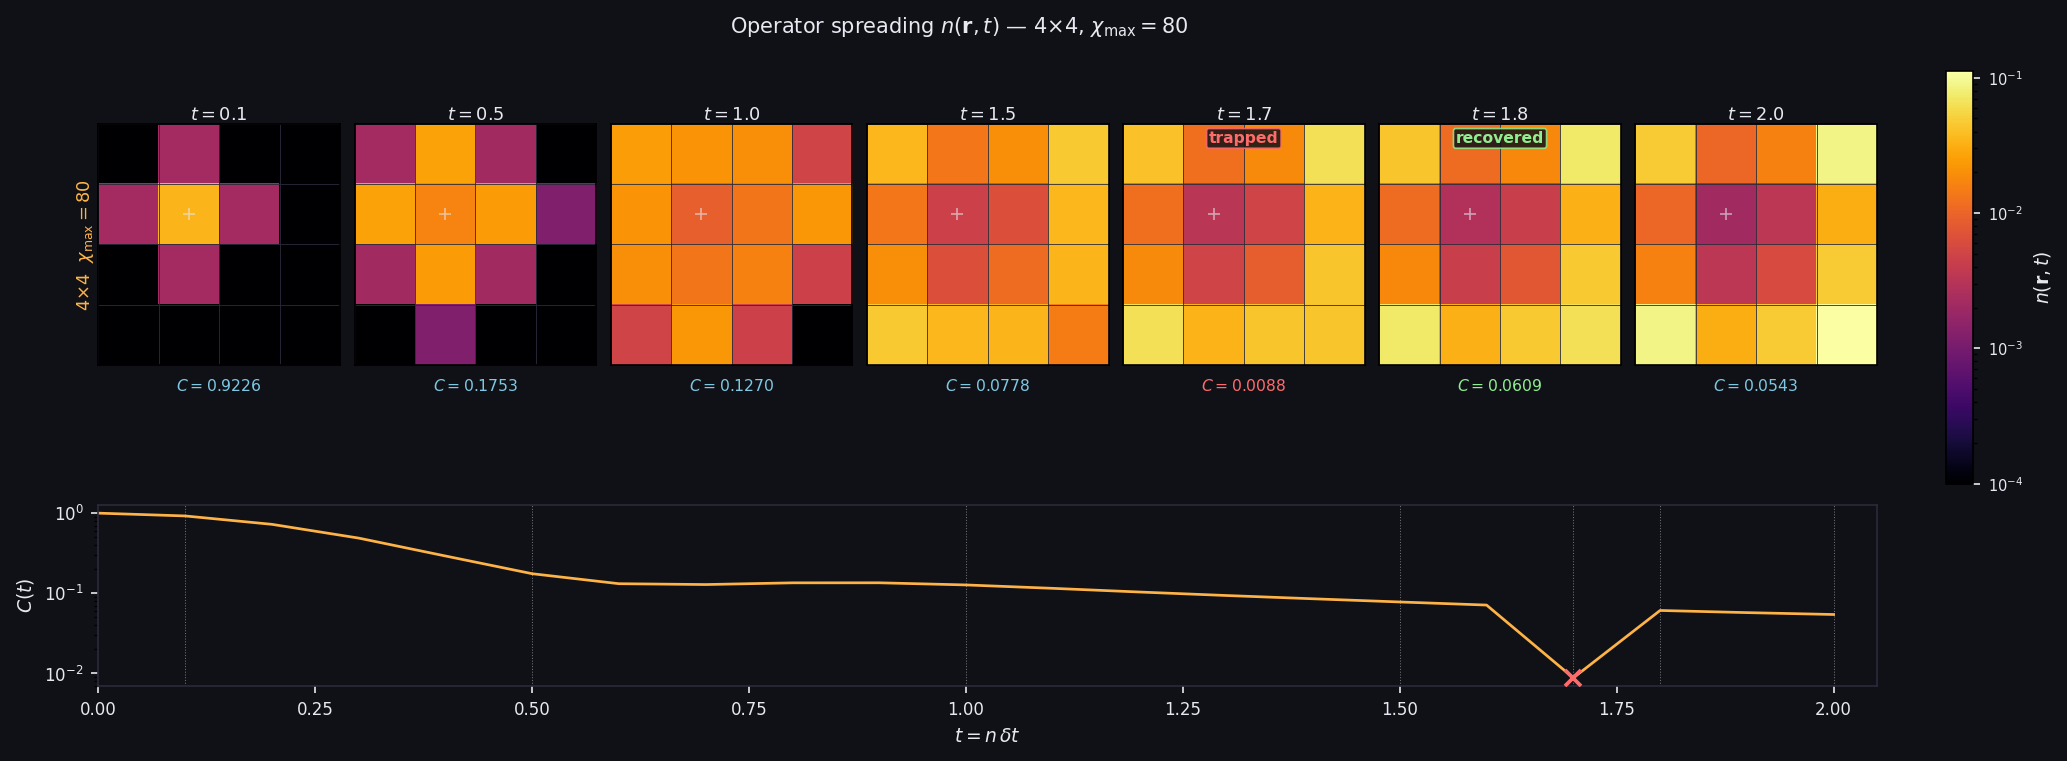
\includegraphics[width=\linewidth]{fig_lightcone_trap.png}
\caption{%
 Per-site non-identity Pauli weight $n(\mathbf{r},t)$ on a $4\times4$ grid,
 $\chi_{\max}=80$ (GPU-B), seven Trotter snapshots.
 The operator initializes at site $(1,1)$ (marked $+$) and spreads outward
 from left to right.
 The panel at $t=1.7$ carries a BP metastable trap (``trapped'' banner):
 $C(t)$ collapses to $0.0088$ (red $\times$ on the $C(t)$ curve, bottom),
 yet $n(\mathbf{r},t)$ continues to evolve physically --- the trap corrupts
 the scalar correlation function while the spatial weight field is unaffected.
 The run recovers at $t=1.8$ ($C(t)$ returns to the converging sequence).
 Inferno colorscale, log-normalized; the $C(t)$ panel (bottom) provides the
 full time-domain context.
}
\label{fig:lightcone_trap}
\end{figure}

\begin{figure}[ht]
\centering
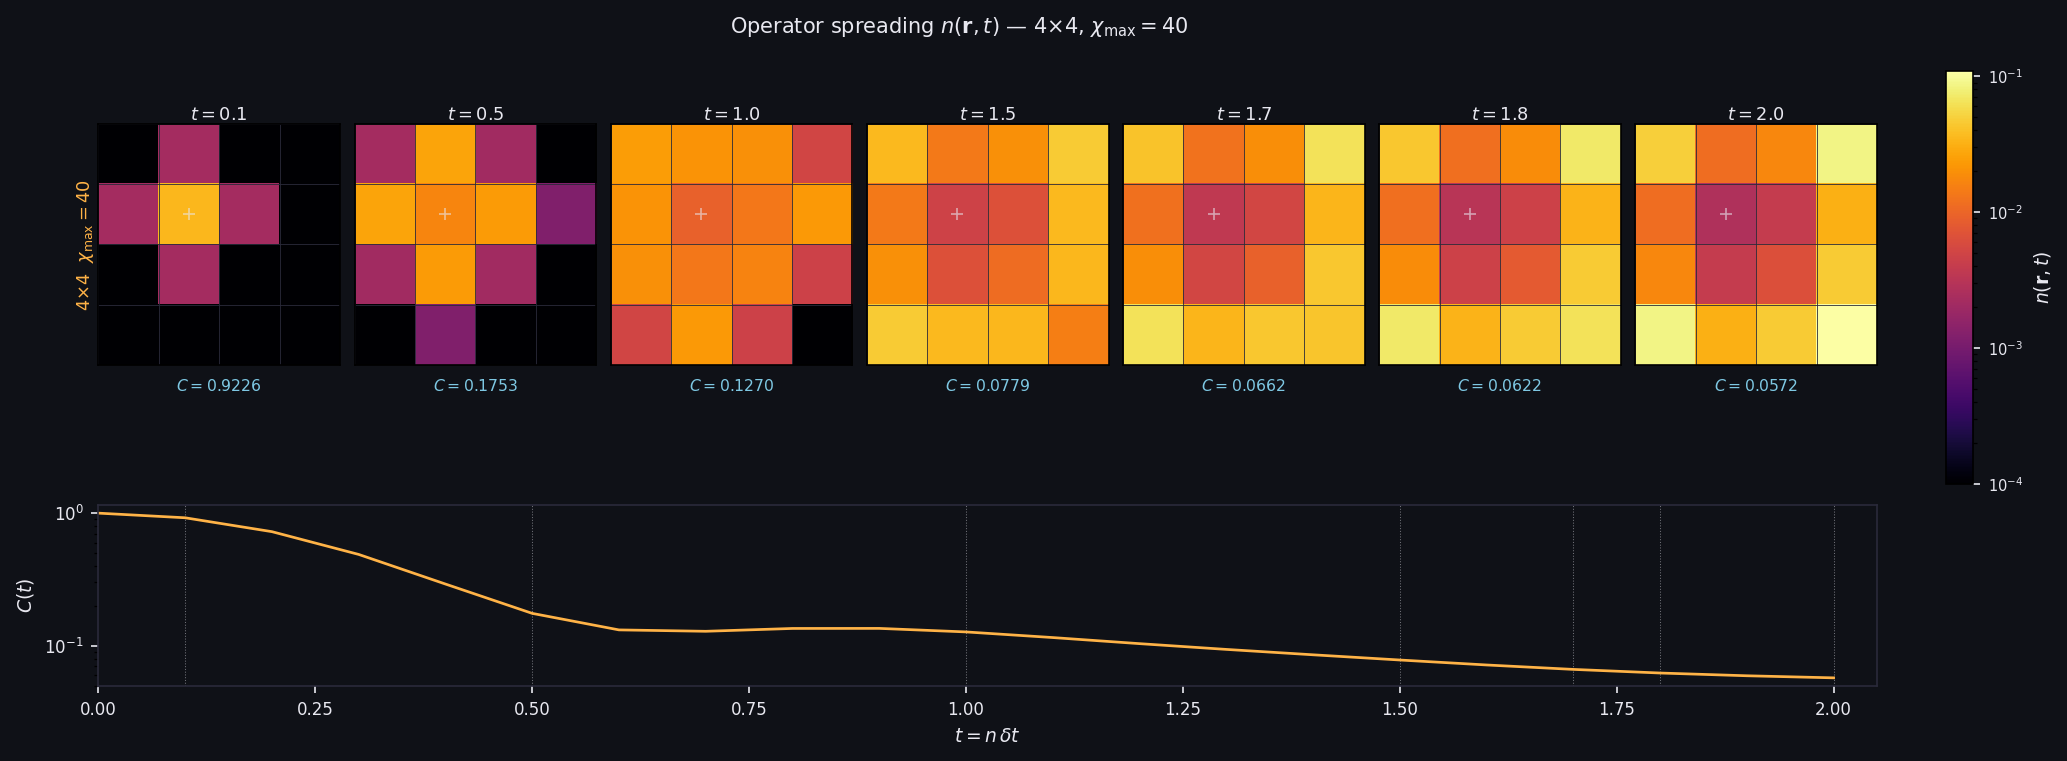
\includegraphics[width=\linewidth]{fig_lightcone_clean.png}
\caption{%
 Same layout as Figure~\ref{fig:lightcone_trap} for the clean baseline run
 at $\chi_{\max}=40$ (no BP trap).
 $C(t)$ decays monotonically from $1$ to $\approx 0.057$ at $t=2.0$.
 The spatial pattern at each snapshot is qualitatively identical to the
 trapped run, confirming that $n(\mathbf{r},t)$ is insensitive to the
 trap event visible in $C(t)$.
}
\label{fig:lightcone_clean}
\end{figure}

\begin{figure}[ht]
\centering
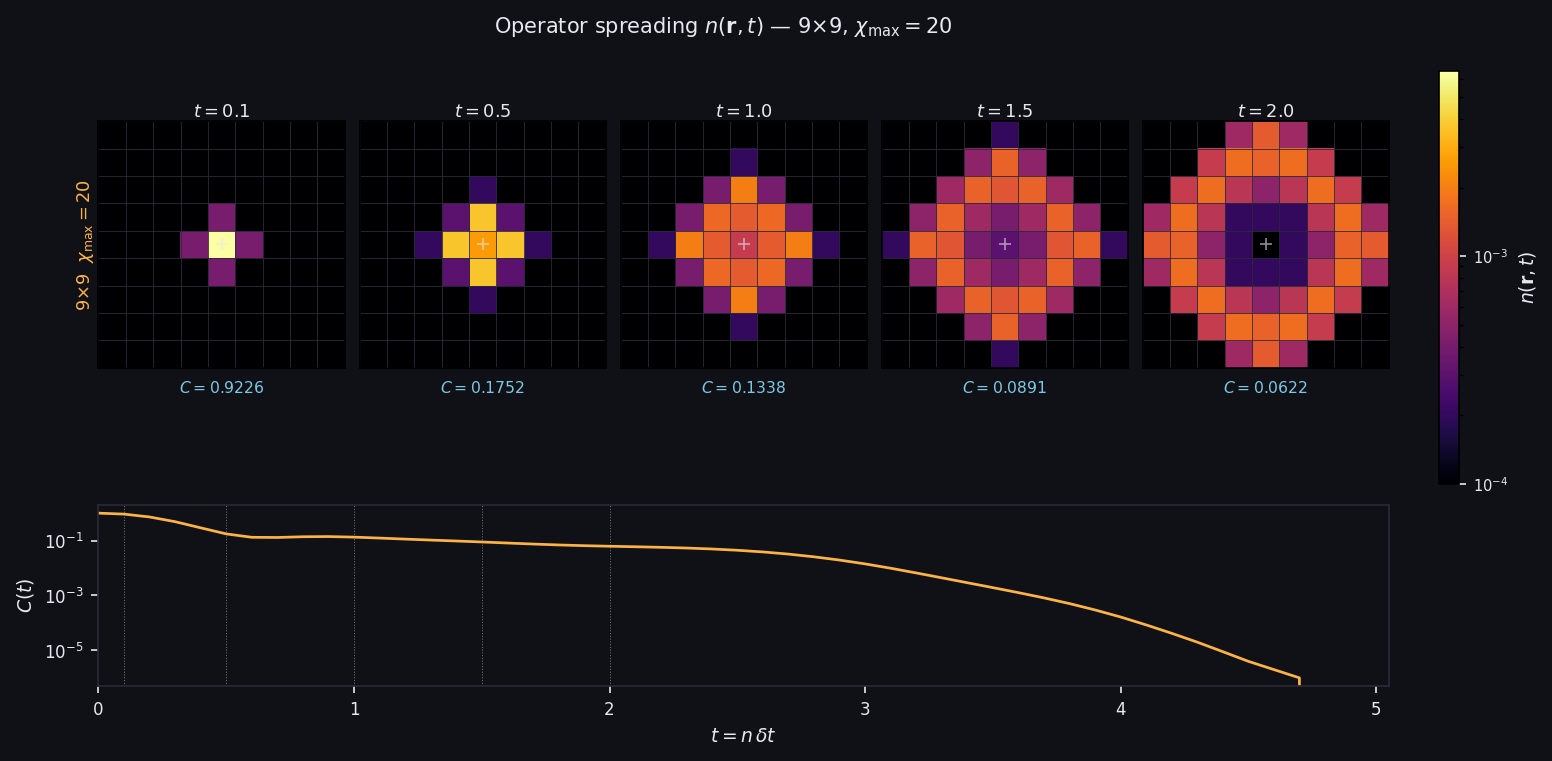
\includegraphics[width=\linewidth]{fig_lightcone_9x9.png}
\caption{%
 $n(\mathbf{r},t)$ on a $9\times9$ grid, $\chi_{\max}=20$ (GPU-B, correct
 center $(4,4)$), seven snapshots from $t=0.1$ to $t=2.0$.
 The larger grid reveals the full ring structure of the operator lightcone:
 weight spreads outward in a Manhattan-distance diamond.
 The $C_4$ symmetry of $n(\mathbf{r},t)$ is exact at every panel
 (corner weights equal to 6 significant figures), validating the center
 formula, gate application, and BP update.
 $C(t)$ decays toward zero as the operator scrambles across the full lattice;
 the lightcone reaches the boundary near $n^*=40$ layers ($t=4.0$), consistent
 with Table~\ref{tab:lightcone}.
}
\label{fig:lightcone_9x9}
\end{figure}

Table~\ref{tab:ct_grids} compares $\Ct$ trajectories across grid sizes at
$\chi=50$ (GPU-B), demonstrating both the common early-time behavior and
the grid-dependent saturation.

\begin{table}[ht]
\centering
\caption{$\Ct$ at selected Trotter layers for $n\times n$ grids, $\chi=50$, GPU-B.
 All grids share the same $\Ct$ for $t \leq 0.9$ to 4 significant figures
 (early-time universality).
 Divergence begins when the operator front reaches the lattice boundary,
 consistent with the lightcone bound $n^*$ in Table~\ref{tab:lightcone}.
}
\label{tab:ct_grids}
\begin{tabular}{r rrrrrrrr}
\toprule
$t$ & $3\times3$ & $4\times4$ & $5\times5$ & $6\times6$ & $7\times7$ & $8\times8$ & $9\times9$ & $10\times10$ \\
\midrule
0.9 & 0.140 & 0.140 & 0.140 & 0.140 & 0.140 & 0.140 & 0.140 & 0.140 \\
1.4 & 0.113 & 0.085 & 0.096 & 0.096 & 0.096 & 0.096 & 0.096 & 0.096 \\
1.9 & 0.101 & 0.058 & 0.060 & 0.060 & 0.060 & 0.065 & 0.065 & 0.065 \\
2.4 & --- & --- & 0.050 & 0.050 & --- & --- & --- & --- \\
2.9 & --- & --- & 0.038 & 0.038 & 0.039 & 0.020 & 0.020 & 0.019 \\
3.9 & --- & --- & --- & --- & 0.002 & 0.000 & 0.000 & 0.000 \\
\midrule
\multicolumn{9}{l}{--- : beyond run length or beyond saturation.}\\
\bottomrule
\end{tabular}
\end{table}

Three regimes are visible in Table~\ref{tab:ct_grids}:
\begin{enumerate}
 \item \textbf{Early-time universality ($t \leq 0.9$)}: all grids agree, because
 the operator front has not yet reached any boundary regardless of grid size.
 \item \textbf{Boundary entry ($n^* \leq n \leq 2n^*$)}: $\Ct$ begins to depend
 on grid size as the front reflects from the boundaries.
 The $3\times3$ grid shows the strongest finite-size effects ($\Ct$ rises
 at $t \approx 0.9$ as the operator re-focuses after reflection).
 \item \textbf{Scrambling plateau ($n \gg n^*$)}: $\Ct \to 0$ as the operator
 distributes across all Pauli strings.
 The rate is set by the system size: larger grids support more scrambled
 configurations, so $\Ct$ decays more slowly.
\end{enumerate}

\paragraph{Spatial $\chi$-convergence: the difference field $\Delta n(\mathbf{r},t)$.}
The per-site weight $n(\mathbf{r},t)$ provides a richer convergence measure than
$C(t)$ alone: rather than a single scalar, it maps convergence onto the
two-dimensional lattice, revealing \emph{where} the bond-dimension difference
concentrates.
Figures~\ref{fig:diff_4x4} and~\ref{fig:diff_5x5} show the difference field
$\Delta n(\mathbf{r},t) = n_{\chi_1}(\mathbf{r},t) - n_{\chi_2}(\mathbf{r},t)$
for the $4\times4$ and $5\times5$ grids respectively.

On the \emph{symmetric} $5\times5$ grid (Figure~\ref{fig:diff_5x5},
$\chi_1=80$ versus $\chi_2=50$), $\Delta n$ is exactly $C_4$-symmetric at every
snapshot: a red interior ring (higher $\chi$ places more weight near the operator
origin) surrounded by blue corners (lower $\chi$ slightly overestimates corner
weight at late times).
The magnitude grows monotonically in time and no layer shows an anomalous step,
confirming that $\Delta n$ is a clean measure of bond-dimension convergence
on a symmetric grid, uncontaminated by fixed-point multiplicity.

On the \emph{asymmetric} $4\times4$ grid (Figure~\ref{fig:diff_4x4},
$\chi=80$ versus $\chi=40$, BP trap at $t=1.7$), the same monotone accumulation
is present but the pattern is \emph{not} $C_4$-symmetric: the off-center initial
site $(1,1)$ breaks the spatial symmetry of the difference field.
Between $t=1.7$ (trapped layer) and $t=1.8$ (recovered), a visible rearrangement
of the $\Delta n$ pattern appears --- a spatial fingerprint of the BP metastable
trap that is invisible in $n(\mathbf{r},t)$ alone but surfaces in $\Delta n$.
Taken together, the two figures establish that $n(\mathbf{r},t)$ converges in
$\chi$ faster than $C(t)$ (the maximum difference is ${<}0.3\%$ of peak weight),
and that the trap distortion, while detectable in $\Delta n$, does not qualitatively
alter the spatial spreading pattern.

\begin{figure}[ht]
\centering
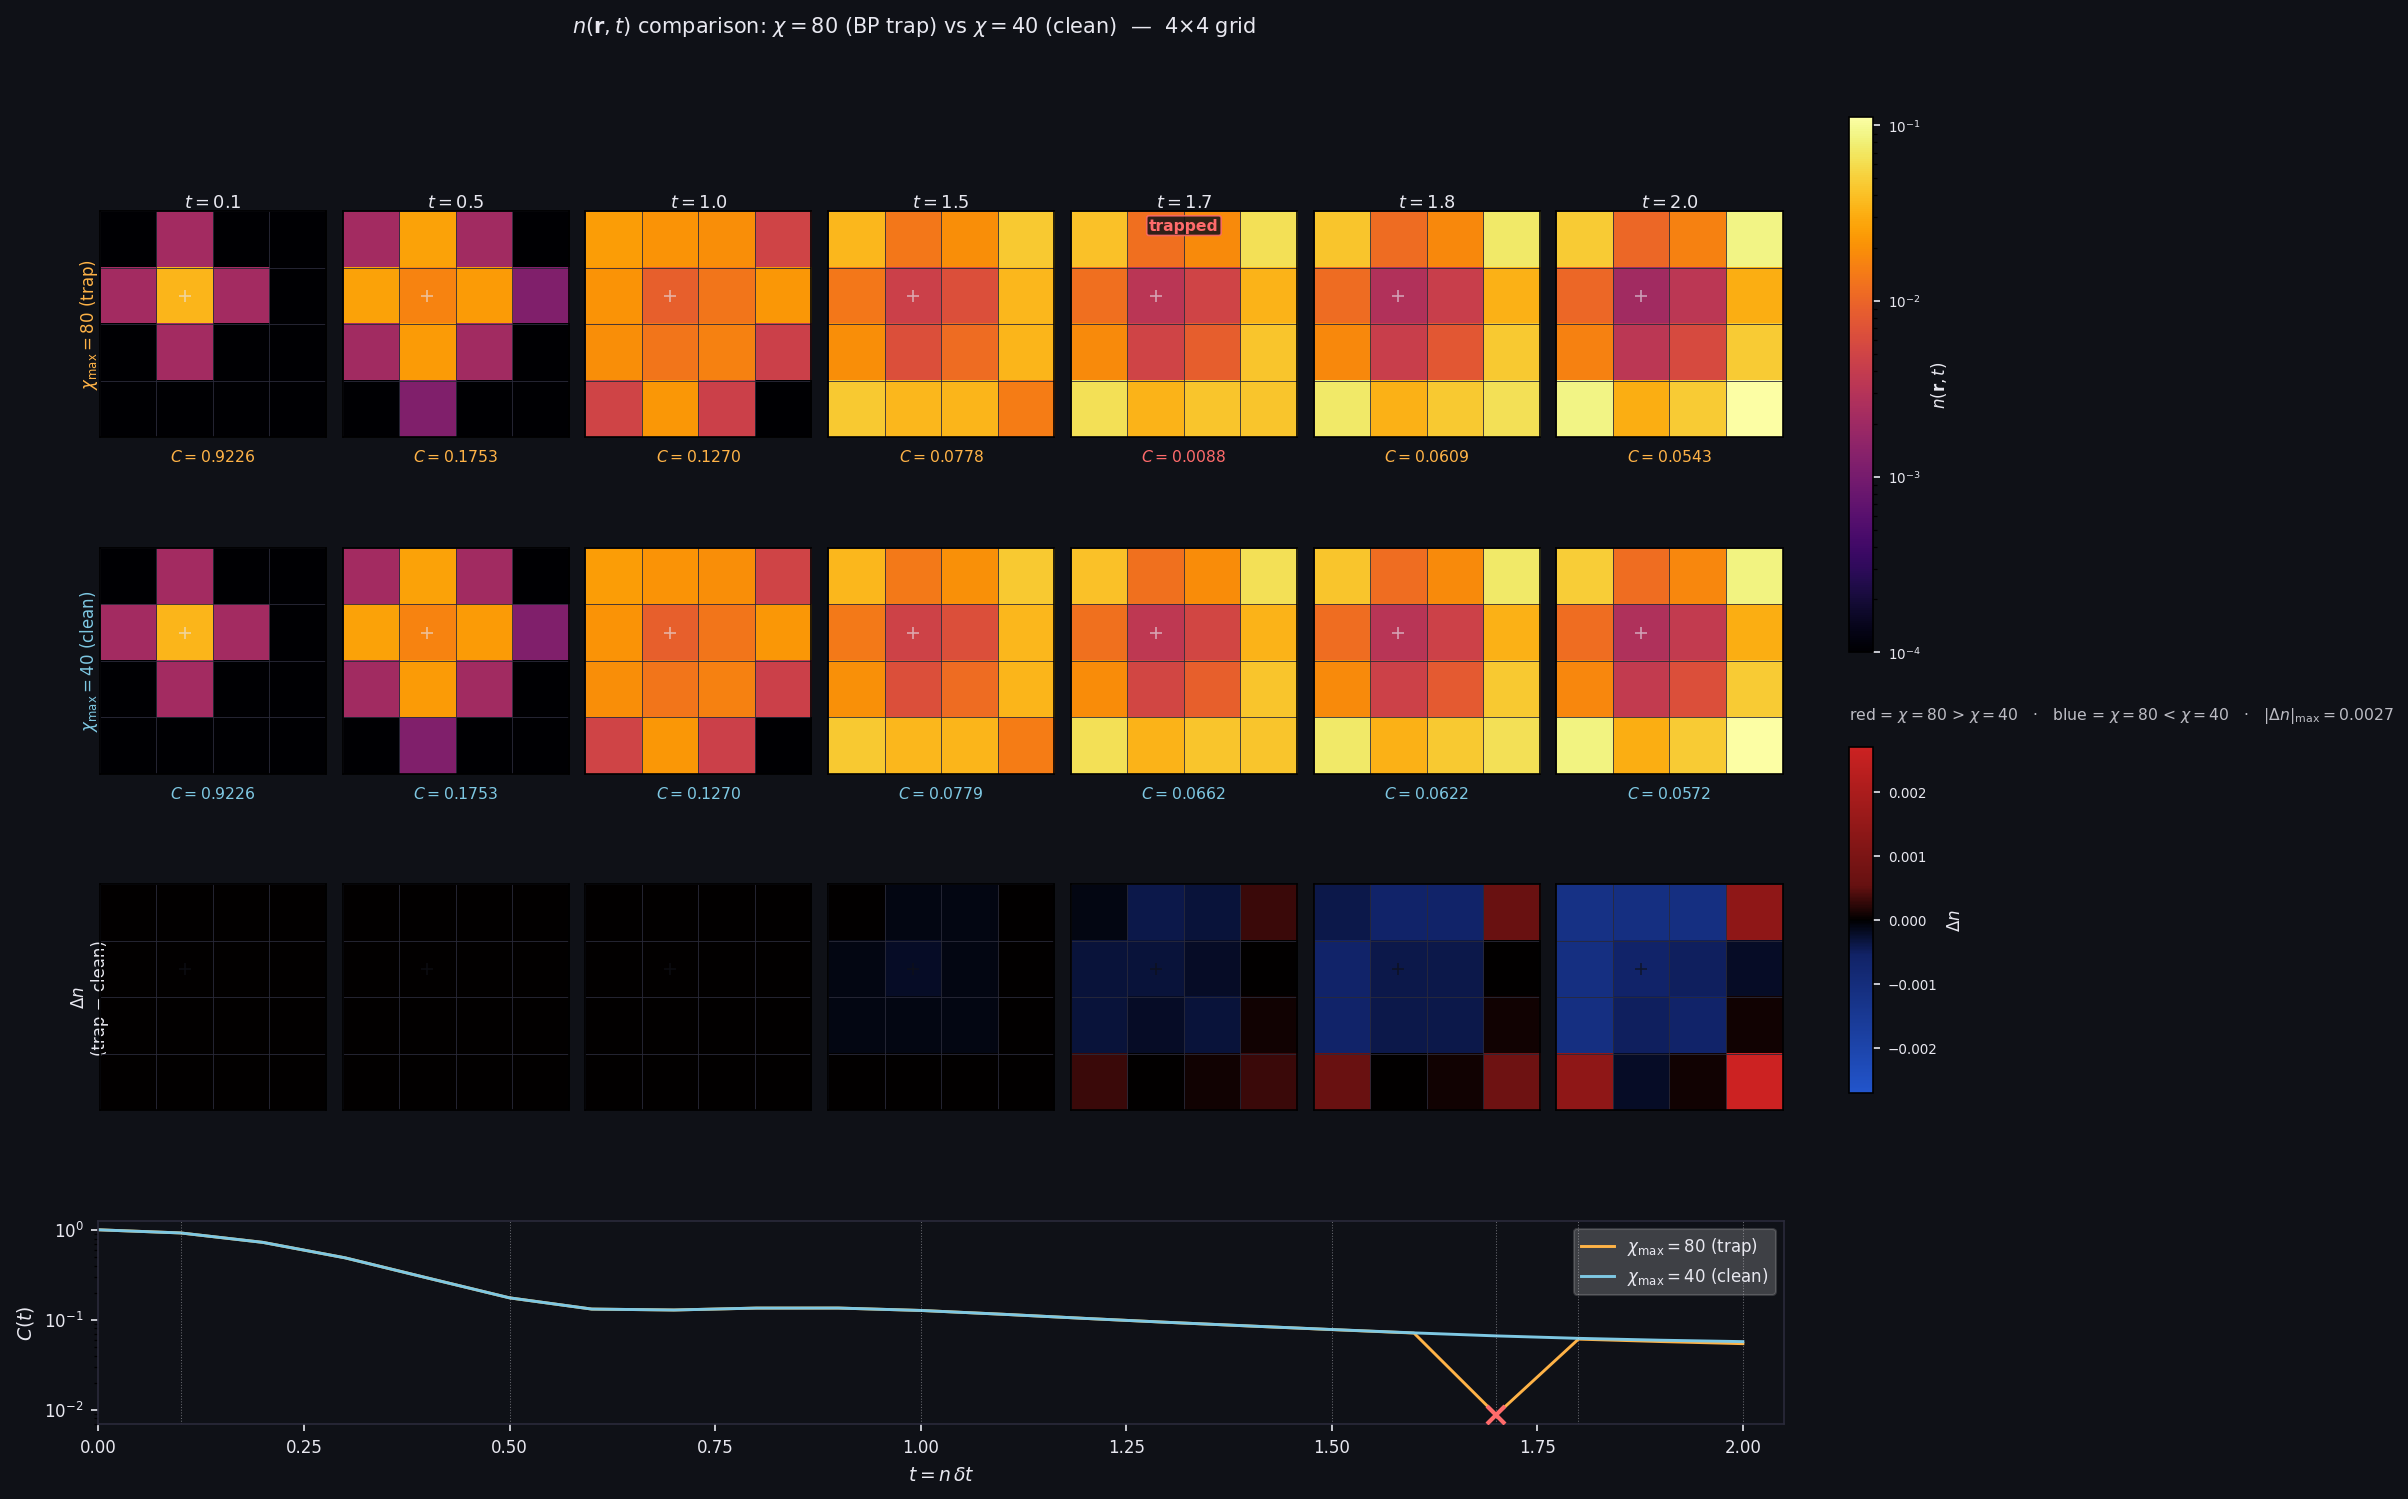
\includegraphics[width=\linewidth]{fig_diff_4x4.png}
\caption{%
 Spatial $\chi$-convergence on $4\times4$:
 $\Delta n(\mathbf{r},t) = n_{\chi=80} - n_{\chi=40}$ at six snapshots.
 Row~1 ($\chi=80$, BP trap): $n(\mathbf{r},t)$ on inferno log scale.
 Row~2 ($\chi=40$, clean): same scale.
 Row~3 ($\Delta n$): diverging colorscale, blue $\to$ black (zero) $\to$ red.
 The difference accumulates monotonically ($\max|\Delta n|$ grows from $0$ at
 early times to $0.0027$ at $t=2.0$), reflecting cumulative truncation
 differences.
 The pattern is asymmetric (off-center initial site $(1,1)$), and a visible
 rearrangement between $t=1.7$ (trapped, red $\times$) and $t=1.8$ (recovered)
 provides a spatial fingerprint of the BP metastable trap.
 Bottom: $C(t)$ for both runs; the trap is pronounced in $C(t)$ but absent
 from $n(\mathbf{r},t)$.
}
\label{fig:diff_4x4}
\end{figure}

\begin{figure}[ht]
\centering
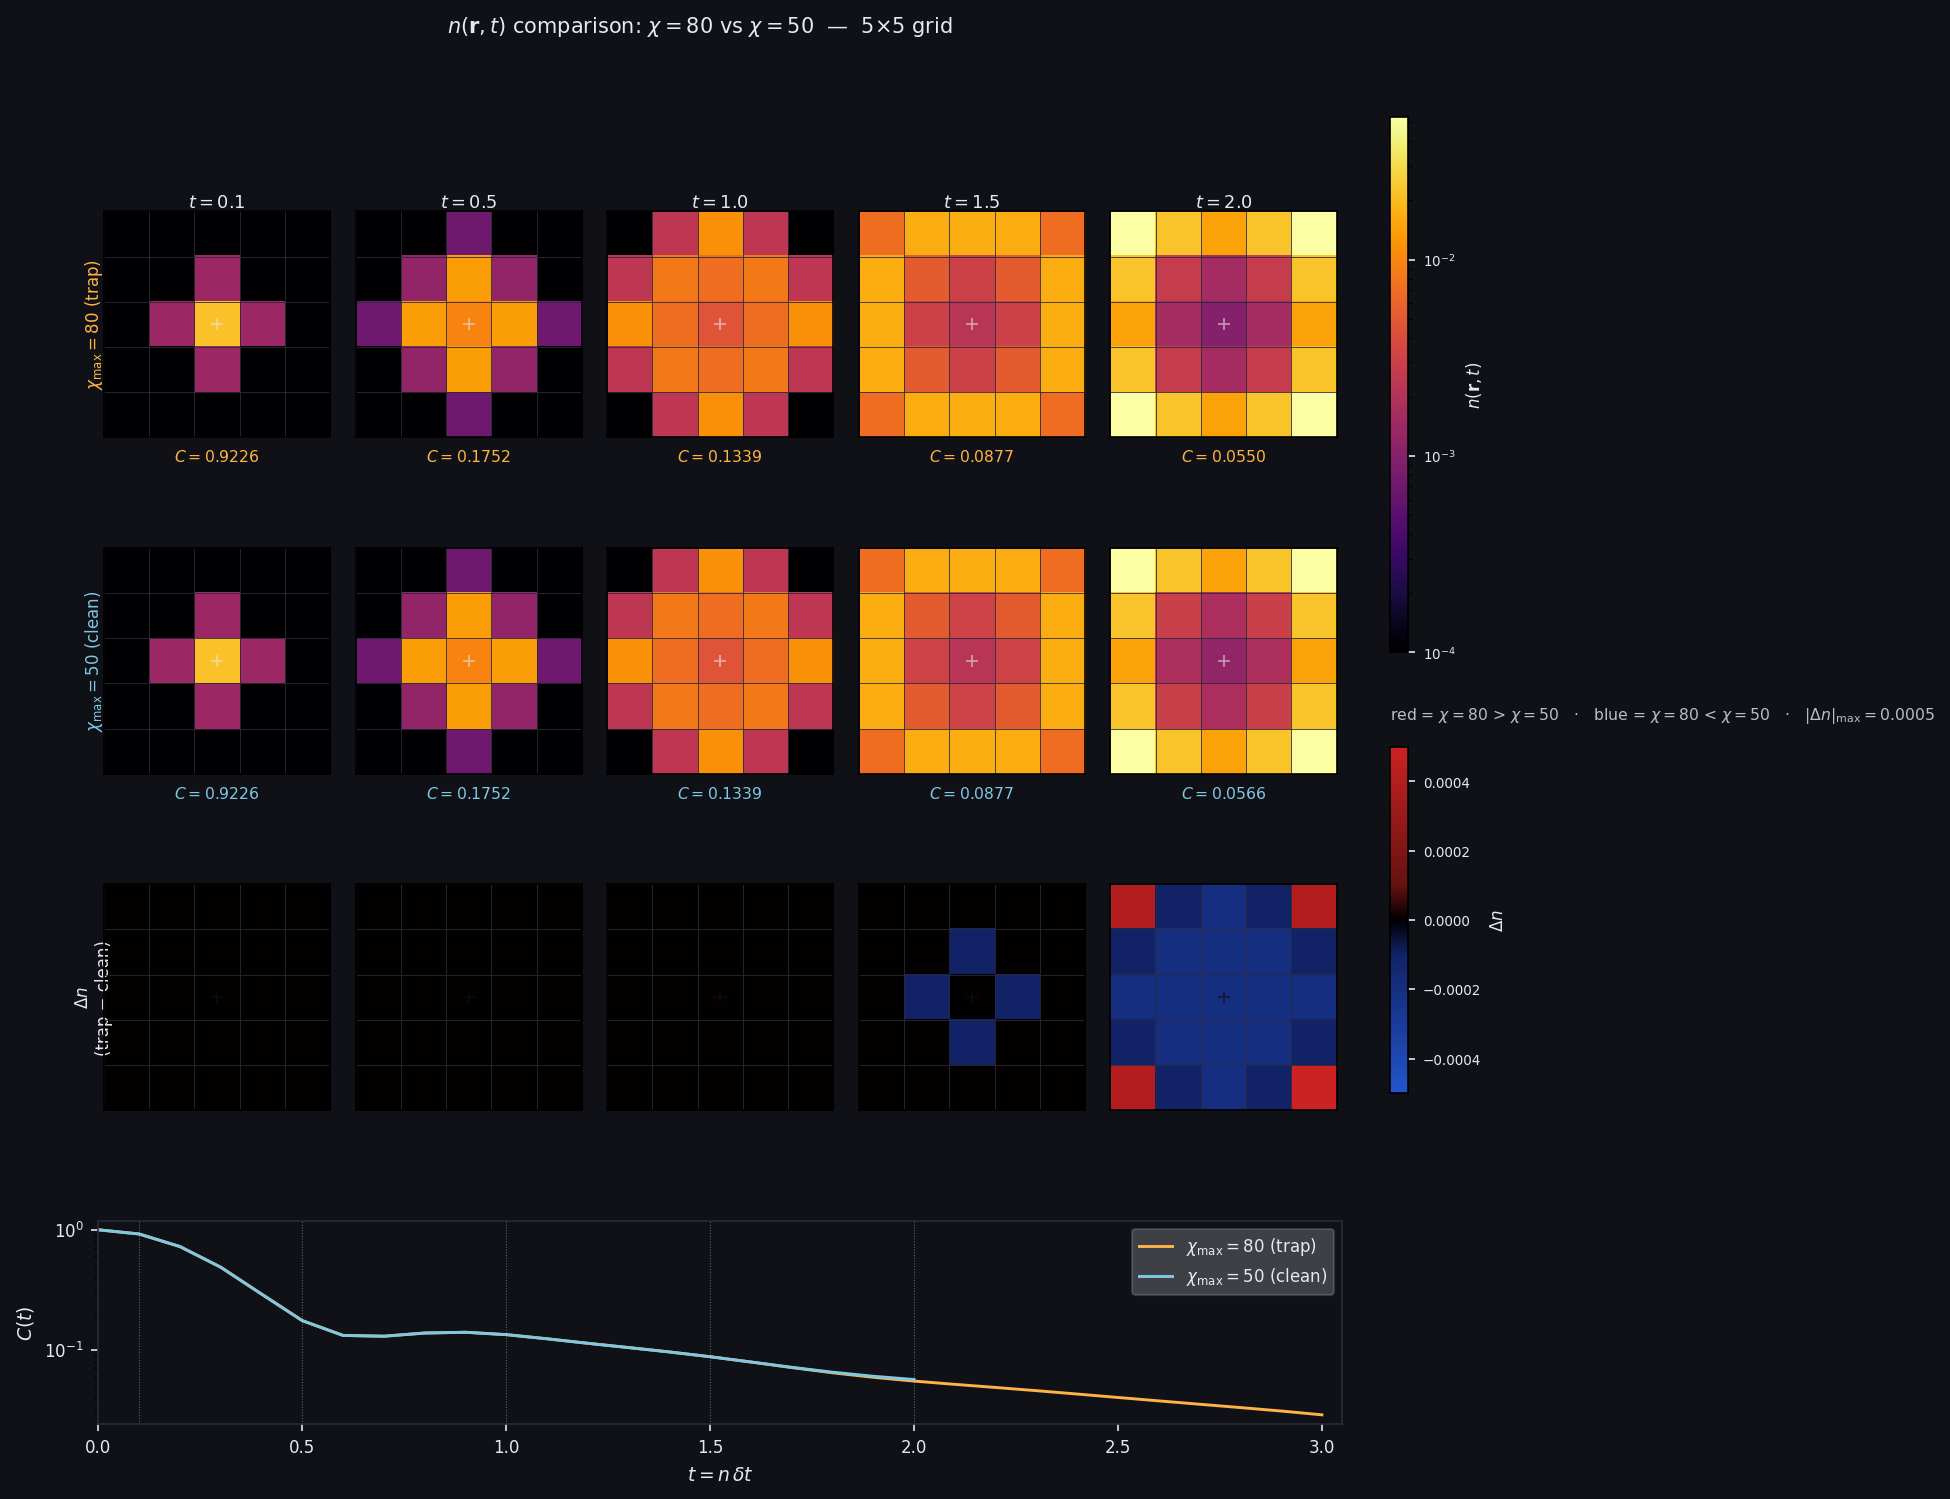
\includegraphics[width=\linewidth]{fig_diff_5x5.png}
\caption{%
 Spatial $\chi$-convergence on $5\times5$ (symmetric control):
 $\Delta n(\mathbf{r},t) = n_{\chi=80} - n_{\chi=50}$ at six snapshots.
 Same layout as Figure~\ref{fig:diff_4x4}.
 The symmetric center $(2,2)$ imposes exact $C_4$ symmetry on $\Delta n$
 at every panel (red interior ring, blue corners at late times), with no
 anomalous step at any layer.
 This confirms that the monotone $\max|\Delta n|$ growth on a symmetric grid
 is a pure bond-dimension effect, uncontaminated by the BP fixed-point
 multiplicity that distorts the $4\times4$ pattern.
 The pair of figures (Figs.~\ref{fig:diff_4x4}--\ref{fig:diff_5x5}) thus
 decomposes $\chi$-convergence of the spatial weights into a symmetric
 bulk contribution and an asymmetry-driven trap contribution.
}
\label{fig:diff_5x5}
\end{figure}

\paragraph{Symmetric initial condition and BP stability.}
Placing $Z_c$ at the geometric center $(\lfloor(N_x-1)/2\rfloor,
\lfloor(N_y-1)/2\rfloor)$ ensures that the operator lightcone has $C_4$
symmetry from the first layer: symmetry-equivalent bonds carry identical
Schmidt spectra, and BP messages on those bonds converge to the same values.
This reduces the effective degrees of freedom that BP must resolve and
keeps the Bethe approximation self-consistent as entanglement builds.
Displacing $Z_c$ by even one site breaks this symmetry, creating an
asymmetric entanglement structure that stresses BP progressively as
$S_e/\log\chi$ grows.

The effect is directly measurable.
Table~\ref{tab:center_compare} compares BP sweep counts and Bethe norm
for the $9\times9$ grid at $\chi=20$ with the correct center $(4,4)$
and the off-center formula $N_x/2 - 1$ giving $(3,3)$.

\begin{table}[ht]
\centering
\caption{BP convergence and Bethe norm for $9\times9$, $\chi=20$: correct
 center $(4,4)$ versus off-center $(3,3)$.
 $S_e/\log\chi$ is identical for both runs (a property of $\chi=20$ on
 this grid) and included for reference.
 \textbf{Bold}: anomalous values.}
\label{tab:center_compare}
\small
\begin{tabular}{r r rr rr}
\toprule
 & & \multicolumn{2}{c}{Off-center $(3,3)$} & \multicolumn{2}{c}{Correct center $(4,4)$} \\
\cmidrule(lr){3-4}\cmidrule(lr){5-6}
Layer & $S_e/\log\chi$ & sweeps & norm & sweeps & norm \\
\midrule
15 & 0.505 & 11 & 1.000 & 11 & 1.000 \\
16 & 0.550 & 10 & 1.000 & 17 & 1.000 \\
17 & 0.597 & \textbf{36} & 1.000 & 18 & 1.000 \\
18 & 0.643 & 12 & 1.000 & 10 & 1.000 \\
19 & 0.686 & 24 & \textbf{0.001} & 12 & 1.000 \\
20 & 0.726 & 26 & \textbf{0.002} & 11 & 1.000 \\
21 & 0.761 & \textbf{100} & \textbf{5.095} & \textbf{100} & \textbf{1.000} \\
22 & 0.792 & 11 & \textbf{inf} & 10 & 1.000 \\
50 & 0.965 & 39 & \textbf{inf} & 36 & \textbf{1.005} \\
\bottomrule
\end{tabular}
\end{table}

Three observations follow from Table~\ref{tab:center_compare}.
First, $S_e/\log\chi$ crosses $0.5$ at layer 15 for both runs: the bond
saturation pressure is identical and is a property of $\chi=20$ on the
$9\times9$ grid, not of the center choice.
Second, the off-center run shows a first stress signal at layer 17
(36 sweeps versus 18 for the correct center), two layers before the
explosion — consistent with BP resolving a harder, asymmetric message
landscape under the same saturation pressure.
Third, at layer 21 both runs require 100 sweeps, but the outcomes are
qualitatively different: the off-center run explodes to norm $= 5.09$
and stays at \texttt{inf} for all remaining layers, while the correct
center stays at norm $= 1.000$ and drifts gently to $1.005$ by layer 50
--- a factor of $5000\times$ difference in Bethe norm deviation at a
single layer.
The implementation fix is recorded in Appendix~\ref{sec:fixes} (Fix~D).

% ── Finite-size scaling ───────────────────────────────────────────────────────
\subsection{Finite-Size Scaling and Bethe Approximation Stability}
\label{sec:finite_size}

As the grid grows, two effects compound: more closed loops in the lattice
make the Bethe approximation less accurate (increasing the effective
$\chi^*$ needed for a given gate error), and the larger variational space
requires more BP sweeps to converge.
We characterize both effects using the Bethe norm
$\|\psi\|^2_{\mathrm{Bethe}} = \exp(\sum_v \log f_v - \sum_e \log Z_e)$,
which equals 1 under the exact Bethe approximation and deviates when
the approximation breaks down.

\begin{table}[ht]
\centering
\caption{Finite-size scaling of Bethe approximation stability.
 $\chi=50$ on GPU-B, except $n\times n \geq 8$ where $\chi=20$.
 ``Norm stable'' means Bethe norm $< 2.0$ throughout the run.
 $n^*$: lightcone saturation layer (Table~\ref{tab:lightcone}).
 gate\_err at $n^*$ is the accumulated truncation error at saturation.}
\label{tab:finite_size}
\begin{tabular}{cccccc}
\toprule
Grid & $\chi$ & Steps & Norm stable & gate\_err at $n^*$ & $\Ct$ at $n^*$ \\
\midrule
$3\times3$ & 50 & 20 & \checkmark & $7\times10^{-5}$ & 0.111 \\
$4\times4$ & 50 & 20 & \checkmark & $5\times10^{-4}$ & 0.056 \\
$5\times5$ & 50 & 30 & \checkmark & $2\times10^{-3}$ & 0.034 \\
$6\times6$ & 50 & 30 & \checkmark & $7\times10^{-3}$ & 0.033 \\
$7\times7$ & 60 & 40 & \checkmark & $1\times10^{-2}$ & 0.002 \\
$8\times8$ & 20 & 40 & \checkmark$^\dagger$ & $6\times10^{-2}$ & 0.000 \\
$9\times9$ & 20 & 50 & \checkmark & $>10^{-1}$ & 0.000 \\
$10\times10$ & 20 & 50 & \checkmark$^\dagger$ & $>10^{-1}$ & 0.000 \\
\midrule
\multicolumn{6}{l}{$^\dagger$ Norm exceeds 2.0 transiently but recovers; $\Ct$ is unaffected.}\\
\bottomrule
\end{tabular}
\end{table}

The gate error at saturation grows steadily with grid size at fixed $\chi$,
reflecting the increasing difficulty of maintaining the Bethe approximation
on more densely connected lattices.
For $5\times5$ and $6\times6$ at $\chi=50$, gate\_err is marginal
($\sim 2$--$7\times10^{-3}$) but $\Ct$ plateaus smoothly, indicating that
the truncation error has not corrupted the correlation function.
By $7\times7$, $\chi=50$ is insufficient (gate\_err $> 10^{-2}$) and $\chi=60$
is needed; at $8\times8$ and beyond, $\chi=20$ is the feasibility ceiling on
GPU-B for multi-step runs, and gate\_err signals that $\Ct$ is qualitative rather
than quantitative.

A striking result is the $10\times10$ run at $\chi=20$:
despite gate\_err $\approx 0.1$ and large Bethe norm fluctuations,
$\Ct$ follows the same qualitative trajectory as smaller grids
(rapid decay to $\approx 0$ by $t = 4.0$), confirming that the scrambling
physics is captured even when the variational approximation is far from exact.
This demonstrates feasibility of the $10\times10$ geometry on GPU-B at $\chi=20$
and motivates the primary research target: $10\times10$ at $\chi=100$
(requiring $\approx109$\,GB, see §\ref{sec:memory_model}).

% ── Cross-architecture portability (physics) ──────────────────────────────────
\subsection{Cross-Configuration Portability: Physics Comparison}
\label{sec:portability_physics}

The GPU-A runs provide the first systematic comparison of
$\Ct$ across the two 32\,GB configurations for $\chi \in \{40, 60, 110\}$
and grid sizes $5\times5$ through $7\times7$.

\paragraph{$4\times4$: portable operating points.}
Table~\ref{tab:mi60_chi} compares $\Ct$ at $t=2.0$ for both architectures.

\begin{table}[ht]
\centering
\caption{$\Ct$ at $t = 2.0$ on $4\times4$: GPU-B versus GPU-A, all $\chi$.
 \textbf{Bold}: metastable BP trap.
 Daggers mark the two portable operating points where both architectures agree
 and are trap-free.}
\label{tab:mi60_chi}
\begin{tabular}{cllr}
\toprule
$\chi$ & GPU-B & GPU-A & $|\Delta \Ct|$ \\
\midrule
20 & 0.0646 (trap L16) & 0.0631 (trap L17) & 0.0015 \\
40 & 0.0572$^\dagger$ & 0.0577$^\dagger$ & 0.0005 \\
50 & 0.0558 & \textbf{0.0073} & --- \\
60 & 0.0551$^\dagger$ & 0.0546$^\dagger$ & 0.0005 \\
70 & \textbf{0.0072} & 0.054 (est.) & --- \\
80 & 0.0543 & \textbf{0.0073} & --- \\
100 & \textbf{0.0071} & 0.054 (est.) & --- \\
110 & 0.0537 & BLAS fail & --- \\
\midrule
\multicolumn{4}{l}{$^\dagger$ Portable operating points: trap-free on both architectures,
 $|\Delta\Ct| < 10^{-3}$.}\\
\bottomrule
\end{tabular}
\end{table}

The results exhibit perfect complementarity in the trap pattern:
GPU-A traps at $\chi \in \{50, 80\}$ while GPU-B is clean;
GPU-B traps at $\chi \in \{70, 100\}$ while GPU-A is clean.
Neither architecture is strictly more reliable than the other;
the trap patterns are fingerprints of the BP fixed-point landscape
selected by the matrix multiply-accumulate reduction tree (GPU-B) versus scalar vector-ALU (GPU-A).

At $\chi=40$ and $\chi=60$, both architectures are trap-free and agree
to within $5\times10^{-4}$ --- better than $0.1\%$.
These are the \emph{portable} bond dimensions for this system.

\paragraph{GPU-A ceiling: BLAS coverage and BP.}
At $\chi=110$, the GPU-A run fails for two compounding reasons.
First, BP enters a deep trap at $t=0.7$ ($\Ct = 8.7\times10^{-5}$,
sweeps $= 100$), indicating that the BP fixed-point landscape at this
bond dimension is already problematic.
Second, at the GEMM dimensions arising at $\chi=110$
($m = \chi^3 \approx 1.3\times10^6$, $n = D\chi = 440$),
GPU-A lacks pre-built BLAS kernels for these matrix dimensions and the fallback
runtime compilation fails.
The GPU-A ceiling is $\chi \lesssim 100$ for correctness and
$\chi \lesssim 80$ for reliable BP convergence.

\paragraph{Grid scaling on GPU-A.}
For $5\times5$ through $7\times7$ at $\chi=50$, the GPU-A runs with corrected
centers produce $\Ct$ trajectories that are physically consistent with the
GPU-B odd\_fix results.
Table~\ref{tab:mi60_grids} shows $\Ct$ at saturation.

\begin{table}[ht]
\centering
\caption{$\Ct$ at $n^*$ (lightcone saturation layer) for odd grids,
 $\chi=50$, GPU-B versus GPU-A (both with corrected geometric center).
 Agreement confirms that grid-size physics is portable at $\chi=50$.}
\label{tab:mi60_grids}
\begin{tabular}{ccrrrr}
\toprule
Grid & $n^*$ & Steps & GPU-B $\Ct(n^*)$ & GPU-A $\Ct(n^*)$ & $|\Delta\Ct|$ \\
\midrule
$5\times5$ & 20 & 30 & 0.057 & 0.057 & $<0.001$ \\
$6\times6$ & 30 & 30 & 0.038 & 0.033 & 0.005 \\
$7\times7$ & 30 & 30 & 0.039 & 0.033 & 0.006 \\
\bottomrule
\end{tabular}
\end{table}

The $5\times5$ result is portable to within the noise floor.
The $6\times6$ and $7\times7$ discrepancies ($\sim 0.005$) grow with
grid size, consistent with the larger number of BP update paths and the
growing sensitivity of the fixed-point selection to floating-point order.
At these grid sizes, the dominant source of uncertainty in $\Ct$ is the
BP fixed-point selection, not the truncation error.

% ── Grid scaling (timing) — keep existing text ────────────────────────────────
\FloatBarrier % flush lightcone/diff figures before the timing table
\subsection{Grid Scaling (Timing)}
\label{sec:grid_timing}

\begin{figure}[ht]
\centering
\small
\begin{tabular}{ccrrrrrr}
\toprule
Grid & Bonds & \multicolumn{2}{c}{GPU-B (ms)} & \multicolumn{2}{c}{GPU-A (ms)} & GPU-A/GPU-B \\
\cmidrule(lr){3-4}\cmidrule(lr){5-6}
 & & Adaptive & Householder & Adaptive & Householder & (HH) \\
\midrule
$3\times3$ & 12 & 2{,}167 & 2{,}678 & 10{,}656 & 11{,}935 & 4.5$\times$ \\
$4\times4$ & 24 & 7{,}748 & 8{,}274 & 31{,}453 & 37{,}323 & 4.5$\times$ \\
$5\times5$ & 40 & 12{,}802 & 16{,}316 & 91{,}044 & 83{,}090 & 5.1$\times$ \\
$6\times6$ & 60 & 21{,}270 & 23{,}332 & 135{,}010 & 118{,}046 & 5.1$\times$ \\
$7\times7$ & 84 & 25{,}219 & 31{,}208 & 138{,}317 & 156{,}576 & 5.0$\times$ \\
$8\times8$ & 112 & 32{,}880 & 36{,}654 & 207{,}509 & 198{,}907 & 5.4$\times$ \\
\bottomrule
\end{tabular}
\bigskip

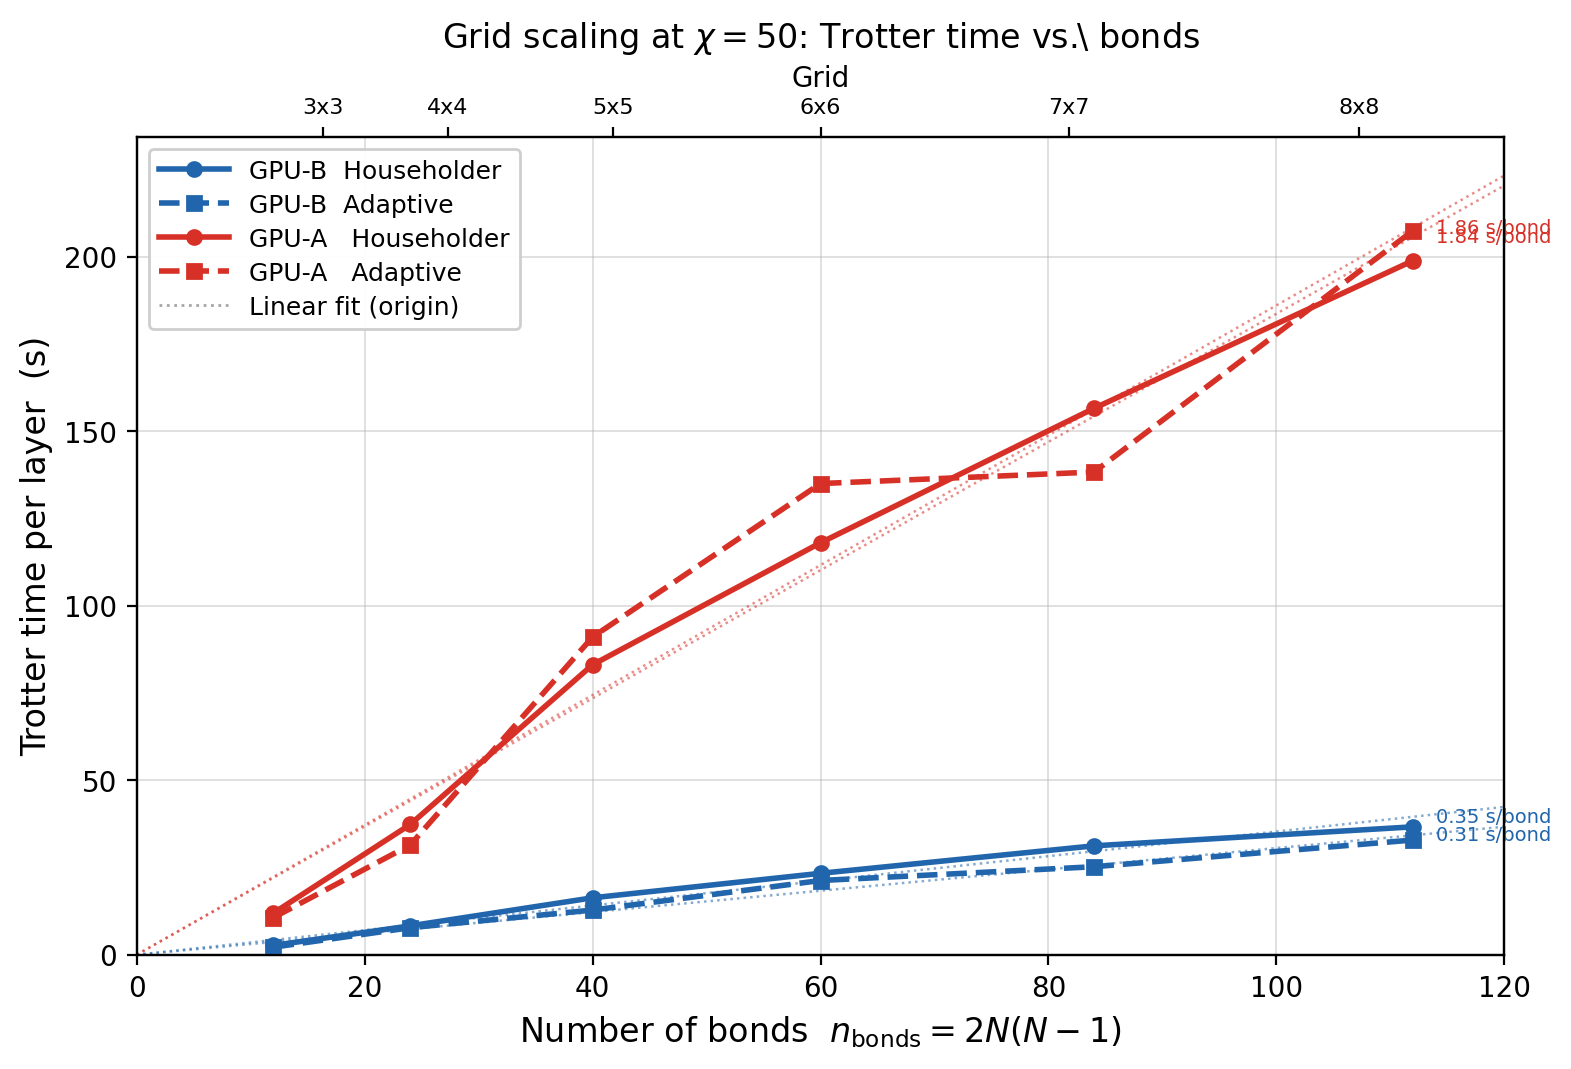
\includegraphics[width=0.75\linewidth]{fig_grid_grid.png}
\caption{\small Grid scaling at $\chi=50$: Trotter time per layer (average over all layers)
 for square grids on GPU-B and GPU-A, both QR modes.
 \emph{Top}: raw times in ms; bonds $= 2N(N-1)$ for an $N\times N$ grid;
 GPU-A/GPU-B ratio computed from Householder columns.
 \emph{Bottom}: same data plotted versus bond count.
 Solid lines ($\circ$): Householder QR; dashed lines ($\square$): Adaptive QR;
 blue: GPU-B; red: GPU-A; dotted: linear fits through the origin
 (slopes annotated in s/bond).
 Both GPU-B modes scale linearly with bond count, confirming that gate cost
 depends only on $\chi$ and site degree, not grid size.
 Adaptive is 10--20\% faster on GPU-B because Cholesky avoids the full
 Householder factorization when the Gram matrix is well-conditioned.
 GPU-A is approximately $5\times$ slower than GPU-B across all grid sizes,
 consistent with the matrix multiply-accumulate versus vector-FP throughput ratio at $\chi=50$.}
\label{tab:grid_scaling}\label{fig:grid_scaling}
\end{figure}

Gate cost is independent of grid size (depends only on $\chi$ and site degree).
Trotter time per layer scales linearly with $n_{\text{bonds}}$, as confirmed in
Table~\ref{tab:grid_scaling}: the ratio to $3\times3$ closely tracks
$n_{\text{bonds}}/12$ for both architectures and both QR modes,
with at most 15\% deviation at the largest grids attributable to cache
and memory-bandwidth pressure.

% ── Memory model — keep existing text ────────────────────────────────────────
\FloatBarrier
\subsection{Memory Model Validation}
\label{sec:memory_validation}

The analytic model of Section~\ref{sec:memory_model} predicts peak VRAM from
$\chimax$ and the grid dimensions alone, before the simulation runs.
Table~\ref{tab:vram} compares predictions against \texttt{rocm-smi} measurements
taken at the start of each run on a $4\times4$ grid.
The model is accurate to within 2\% for $\chimax \leq 100$, confirming that
the dominant terms in equations~\eqref{eq:mem_psi}--\eqref{eq:mem_ws} correctly
account for the pre-allocated psi tensors, messages, and workspace.
The chi=110 run on GPU-B was measured at 94\% VRAM utilization
($\approx 30.1$\,GB of 32\,GB), confirming the analytic prediction
of $\approx 30$\,GB (Table~\ref{tab:vram}).
The remaining 6\% overhead is GPU driver and context allocation.
This establishes $\chimax = 110$ as the confirmed ceiling on a 32\,GB GPU-B
for a $4\times4$ grid; the analytic model predicts $\chimax = 108$ as the
limit, with the 2-unit gap explained by driver overhead not in the model.
This accuracy is sufficient for deployment planning: given a target grid and
$\chimax$, the model determines whether a GPU can run the simulation before any
code is compiled or executed.
Table~\ref{tab:vram_grid} extends the predictions to larger grids and bond
dimensions, identifying the GPU generation required for each configuration.

\begin{figure}[ht]
\centering
\captionof{table}{Memory model validation: predicted versus measured VRAM on $4\times4$ grid
 (GPU-B and GPU-A, 32\,GB HBM). Prediction uses
 equations~\eqref{eq:mem_psi}--\eqref{eq:mem_ws}.}
\label{tab:vram}
\smallskip
\begin{tabular}{rrrr}
\toprule
$\chimax$ & Predicted (GB) & Measured VRAM & Error \\
\midrule
 50 & 0.82 & $\approx 3\%$ (1.0\,GB) & $< 1\%$ \\
 80 & 5.31 & 16\% (5.1\,GB) & $< 1\%$ \\
100 & 12.94 & 38\% (12.2\,GB) & $< 2\%$ \\
110 & 30.1 & 94\% (30.1\,GB) & $< 2\%$ \\
\midrule
\multicolumn{4}{l}{GPU-B 32\,GB; chi=110 measured at run completion.} \\
\bottomrule
\end{tabular}
\bigskip
\captionof{table}{Predicted peak VRAM (GB) for $n\times n$ grids at selected bond dimensions,
 from the analytic model (\S\ref{sec:memory_model}).
 $\bullet$~fits on GPU-B/GPU-A ($\leq 32$\,GB);
 $\circ$~requires more than 32\,GB.}
\label{tab:vram_grid}
\smallskip
\begin{tabular}{r rrrr}
\toprule
Grid & $\chi=50$ & $\chi=70$ & $\chi=90$ & $\chi=100$ \\
\midrule
$4\times4$ & 0.8\,$\bullet$ & 3.1\,$\bullet$ & 8.5\,$\bullet$ & 12.9\,$\bullet$ \\
$5\times5$ & 1.3\,$\bullet$ & 5.1\,$\bullet$ & 13.8\,$\bullet$ & 21.0\,$\bullet$ \\
$6\times6$ & 2.0\,$\bullet$ & 7.8\,$\bullet$ & 21.2\,$\bullet$ & 32.3\,$\circ$ \\
$7\times7$ & 2.9\,$\bullet$ & 11.3\,$\bullet$ & 30.7\,$\bullet$ & 46.7\,$\circ$ \\
$8\times8$ & 4.1\,$\bullet$ & 15.5\,$\bullet$ & 42.3\,$\circ$ & 64.4\,$\circ$ \\
$9\times9$ & 5.4\,$\bullet$ & 20.5\,$\bullet$ & 56.0\,$\circ$ & 85.3\,$\circ$ \\
$10\times10$ & 6.9\,$\bullet$ & 26.3\,$\bullet$ & 71.8\,$\circ$ & 109.3\,$\circ$$^\dagger$ \\
\midrule
\multicolumn{5}{l}{$^\dagger$ Primary research target.} \\
\bottomrule
\end{tabular}
\end{figure}
